\documentclass[a4paper,twoside,12pt]{report}

% Import specific style file in this directory
\usepackage{thesis}

%{{{ Alias commands specific to the thesis package
\newcommand{\shortdoctitle}{$E\_r$-Generating Mechanisms}
\newcommand{\doctitle}{Comparing Radial Electric Field-Generating Mechanisms in L--H Transitions}
\newcommand{\docsubtitle}{Master's Thesis}

\newcommand{\me}{Kevin A. Blondino}
\newcommand{\keywords}{H-mode, bifurcation, L-mode, thesis, fusion, tokamak}
\newcommand{\version}{EMPTY version}
\newcommand{\monthYear}{February 2018}

\newcommand{\firstCommitteeMember}{dr. H.J. de Blank}
\newcommand{\secondCommitteeMember}{Second Committee Member}
\newcommand{\thirdCommitteeMember}{Third Committee Member}
%}}}

\title{\doctitle}
\author{\me}

\usepackage{fullpage, indentfirst, graphicx, amsmath, float}
\usepackage{cancel}
\linespread{1.1}
\usepackage[dvipsnames]{xcolor}
\usepackage[labelfont=bf]{caption}
\usepackage[title,titletoc]{appendix}
\usepackage[UKenglish]{isodate}
\cleanlookdateon
\usepackage[T1]{fontenc}
\usepackage[utf8]{inputenc}
\usepackage{cleveref}

% SageTeX!
\usepackage{sagetex}

% Minted package for printing code
% MUST BE COMPILED with -shell-escape flag!
\usepackage{minted}

%{{{ Setup References and hyperref
\usepackage[backend=bibtex, url=false, backref=true]{biblatex}
\addbibresource{../References/References.bib}
\DefineBibliographyStrings{english}{bibliography = {References}}

\usepackage{hyperref}
\hypersetup
{
	unicode=true,%
	bookmarks=true,%
	colorlinks=false,%
	linkbordercolor={0.980 0.500 0.449},%
	citebordercolor={0.449 0.926 0.980},%
	pdfauthor={\me},%
	pdfcreator={\me},%
	pdftitle={\shortdoctitle},%
	pdfsubject={\doctitle},%
	pdfkeywords={\keywords}
}
%}}}

%{{{ Two Figures Side-by-Side, separate captions
%\newsavebox\IBoxA \newsavebox\IBoxB \newlength\IHeight
\newcommand\TwoFig[6]{% Image1 Caption1 Label1 Im2 Cap2 Lab2
%	\sbox\IBoxA{#1}
%	\sbox\IBoxB{#4}%
%	\ifdim\ht\IBoxA>\ht\IBoxB
%		\setlength\IHeight{\ht\IBoxB}%
%	\else\setlength\IHeight{\ht\IBoxA}\fi
	\begin{figure}[hbt]
		\minipage[t]{0.48\textwidth}\centering
			{#1}
			\caption{#2}\label{#3}
		\endminipage\hfill\vrule\hfill
		\minipage[t]{0.48\textwidth}\centering
			{#4}
			\caption{#5}\label{#6}
		\endminipage
	\end{figure}%
}
%}}}

%{{{ Two Figures Side-by-Side, with 1 caption
\newcommand\TwoFigOneCap[4]{% Image1 Im2 Caption Label
%	\sbox\IBoxA{#1}
%	\sbox\IBoxB{#2}%
%	\ifdim\ht\IBoxA>\ht\IBoxB
%		\setlength\IHeight{\ht\IBoxB}%
%	\else\setlength\IHeight{\ht\IBoxA}\fi
	\begin{figure}[hbt]
		\minipage[t]{0.48\textwidth}\centering
			{#1}
		\endminipage\hfill
		\minipage[t]{0.48\textwidth}\centering
			{#2}
		\endminipage
		\caption{#3}\label{#4}
	\end{figure}%
}
%}}}


% Temporary Packages
\usepackage{lipsum}

% ---------------------------------------------------------

\begin{document}
% Number the pages before the start
\pagenumbering{roman}

\begin{titlepage}
\begin{center}
%
\includegraphics[height=2cm]{../Graphics/tue-logo-high}\\

\includegraphics[height=3cm]{../Graphics/tue_fusion_logo}\\
%\LARGE
%Eindhoven University of Technology \\
\large
Department of Applied Physics  \\
Science and Technology of Nuclear Fusion

\vspace*{10cm}

\setlength{\TPHorizModule}{1mm}
\setlength{\TPVertModule}{\TPHorizModule}
% Set the Paragraph Indent to zero, so the first line is not Indented
% Back-up the current value so it can be put back at the end of the title page
\newlength{\backupparindent}
\setlength{\backupparindent}{\parindent}
\setlength{\parindent}{0mm}			
% Begins a textbox at 62 mm from the left of the edge of the paper and 89 mm from the top
% The width of the textbox is 95 mm (167 - 72 mm)
% The height of the box cannot be defined, so it is your task to keep the text not too long
\begin{textblock}{145}(35,89)
	\vspace*{1mm}
	\huge
	\textbf{\doctitle \\}
	\Large
	\vspace*{8mm}
	\textit{\docsubtitle}\\
	\vspace*{15mm}
	\Large
	\me\\
\end{textblock}

\large
Supervisor:\\
\begin{tabular}{rl}
	\firstCommitteeMember\\
\end{tabular}
\\ \vspace*{5mm}
Committee Members:\\\vspace*{2mm}
\begin{tabular}{rl}
	\secondCommitteeMember\\
	\thirdCommitteeMember\\
	\fourthCommitteeMember\\
\end{tabular}

%\vfill
%\version

\vfill
%\docdate \\
\large
Eindhoven, NL\\
\today\\

% Put the Paragraph Indent back to its original value
\setlength{\parindent}{\backupparindent}
\end{center}
\end{titlepage}



\normalsize
\clearemptydoublepage

\chapter*{Abstract}\label{chapter:abstract}
%\input{ABSTRACT FILE HERE!!}
\addcontentsline{toc}{chapter}{Abstract}

\cleardoublepage
\tableofcontents
\cleardoublepage

% ---------------------------------------------------------

\setcounter{page}{0}
\pagenumbering{arabic}
In 1982, a new neutral-beam injection heating system was install in the ASDEX tokamak, which pushed the device into a new realm.
A new level of energy confinement time was achieved, measured to be a factor of 2 or more than what was expected.
This state of operation was coined the high-confinement (H--) mode, and is now considered necessary for the future of nuclear fusion as an energy source \cite{arnoux_how_2009} \cite{wagner_development_1984}.
With this new level of energy confinement, the community got one step closer to economic fusion power plants.
The details of this transition, however, are not fully understood.

\section{Characteristics of L-- and H--Mode}\label{sec:characteristics}
Transport of particles and energy in tokamaks has been discovered to be significantly dominated by anomalous (turbulent) transport, which is generally assumed to be generated by turbulence, which are driven by micro-instabilities.
Low-confinement mode, referred to as L--mode, is dominated by this transport at the edge.
The formation of H--mode is due to the suppression of this turbulent transport at the edge of the plasma.
This mode is therefore categorized as having a transport barrier.
The plasma edge is defined to be the thin boundary layer of the plasma just inside the last-closed flux surface.

\begin{figure}[tb] % L--H-modes compare
\begin{minipage}{0.49\linewidth}
	\centering
	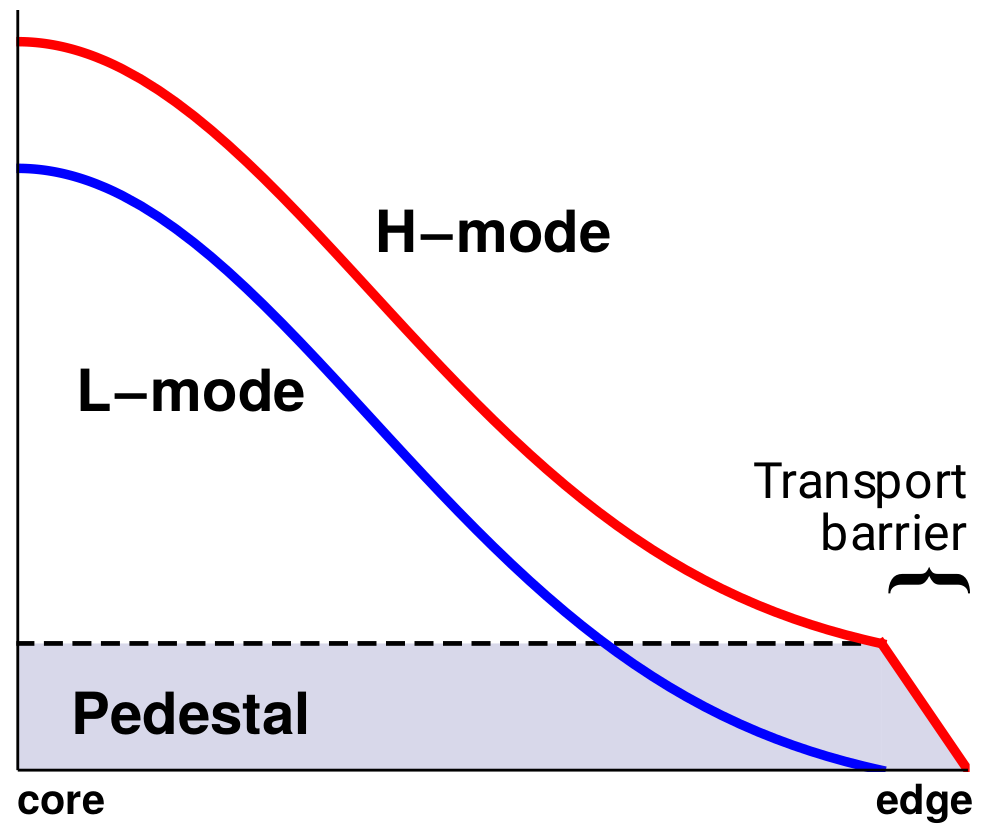
\includegraphics[width=0.8\textwidth]{../Graphics/L-mode_H-mode_compare.png}
\end{minipage}
\hfill
\begin{minipage}{0.49\linewidth}
	\caption{A comparison of the radial pressure profiles of L--mode and H--mode.
	The profile of H--mode can be thought of as on a ``pedestal,'' in which the pressure profile is increase in the core.
	This is due to the transport barrier that is formed at the edge \cite{weymiens_bifurcation_2014}.}
	\label{fig:L-mode_H-mode_compare}
\end{minipage}
\end{figure}

One of the properties of H--mode is its significantly-raised pressure profile compared to that of L--mode, and is said to sit on a ``pedestal.''
Accordingly, there is a steep gradient in the pressure at the edge of the plasma, shown and compared to L--mode in Figure~\ref{fig:L-mode_H-mode_compare} \cite{weymiens_bifurcation_2014}.
This allows for an increased temperature in the core.

In addition, hysteresis is present between the modes, in which the threshold power for the transition between the two modes is based on the current mode.
This is covered in-depth in Section~\ref{ssec:hysteresis}.

\section{The L--H Transition}\label{sec:the_transition}
The key feature that determines a divertor tokamak's operational mode is the amount of external heating power.
Limiter tokamaks are relegated to stay in L--mode, as H--mode is an exclusive operating mode of tokamaks with divertors.
The transition has been observed to occur in one of three general manners: sharp, smooth, and oscillatory.

\subsection{Bifurcation Theory}\label{ssec:bif_theory}
The aforementioned transitions show clear evidence of bifurcations in the plasma system.
%A defining feature of L--H transitions is that they can occur very suddenly (the so-called sharp transition), which is characteristic of fold bifurcation behavior.
Mathematically, a bifurcation is defined to be a topological or qualitative change in a system when a small and smooth change of a parameter is made.
A simple example for a fold bifurcation is the following, with $a$ representing the parameter:
\begin{equation} % Simplest fold bifurcation
	\frac{\text{d}x}{\text{d}t} \,=\, \dot{x} \,=\, a + x^2.
	\label{eq:simple_fold}
\end{equation}
This equation can behave in one of three manners:
If $a > 0$, there are no real points of equilibrium, also known as steady-state solutions.
For $a = 0$, there is one equilibrium point at $x = 0$, and two for $a < 0$, at $x = \pm\sqrt{-a}$.
Varying $a$ from some positive real number to some negative number, the fundamental behavior of the solutions changes drastically at $a = 0$ with the sudden appearance of a steady-state solution.
Equation~\ref{eq:simple_fold} is the simplest known form of a fold bifurcation, also known as the saddle-node bifurcation.
The simplest form for any dynamical system is known as the topological norm form.
A parameter plot of $x$ versus $a$ in Fig.~\ref{fig:simple_fold} illustrates this, with the green and red curves representing the stable and unstable steady-state solutions, respectively.

%{{{ Two figures for simple bifurcations (co-dimension 1 and 2)
\TwoFig{../Graphics/Bif_Graphs/Simple_fold.png}
	{Plot of parameter space for $\dot{x} = a + x^2$ (Eq.~\ref{eq:simple_fold}), with the co-dimension 1 bifurcation occurring at $a = 0$. %
	For $a < 0$, the system has two steady-state solutions; the green is stable, while the red is unstable.
	For $a > 0$, there is no steady-state solution.}
	{fig:simple_fold}
	{../Graphics/Bif_Graphs/co-2_fold.png}
	{Plot of parameter space for $\dot{x} = -(a + x - x^3)$ (Eq.~\ref{eq:sharp_bif}). %
	This system showcases two fold bifurcations (each of co-dimension 1), at the turning points $a_{\pm\text{crit}}$, with two stable regions, in green and blue. %
	The red region is an intermediate that is unstable.}
	{fig:co-2_fold}
%}}}

The co-dimension of a system refers to the lowest number of parameters required to produce the topological norm form.
Put differently, it is the number of parameters that must be varied for the bifurcation to occur.
In the case of Eq.~\ref{eq:simple_fold}, there is only a single parameter, and is thus referred to as a co-dimension 1 bifurcation \cite{weymiens_bifurcation_2014}.

\subsubsection{Sharp and Smooth Transition Bifurcations}
%{{{ Two figures for zeros of the co-dimension 2 bifurcation
\TwoFigOneCap{../Graphics/Bif_Graphs/stationary_b-0_8.png}
	{../Graphics/Bif_Graphs/stationary_b_1_1.png}
	{Phase plots for Eq.~\ref{eq:sharp_bif}, with different values of $a$ within each plot. %
	There is a variance in the number of zeros based on the values of $a$ in the right plot, while there is strictly one zero for all values of $a$ in the left plot. %
	When there is multiple roots, the middle zero is always unstable.}
	{fig:stationaries_b}
%}}}

The dynamic behavior of the L--H transition correspond very closely to a few certain bifurcations.
Sharp and smooth transitions are features of the cusp bifurcation.
The topological norm form of this behavior is
\begin{equation}
	\dot{x} \,=\, -(a + bx - x^3)~.
	\label{eq:sharp_bif}
\end{equation}
Figure~\ref{fig:co-2_fold} is a plot of the parameter space, indicating the stable and unstable steady-state solutions.
This cusp bifurcation can also be regarded as two co-dimension 1 folds, if one views the positive and negative $x$-domains as separate co-dimension 1 bifurcations.
The distinction between sharp and smooth transitions in this co-dimension 2 bifurcation is solely based on the $b$ parameter, shown in the plots of Figure~\ref{fig:Bif_hysteresis}.
As $b$ approaches zero from some positive value, the size of the hysteresis shrinks, with it vanishing at $b = 0$, in which the smooth transition occurs.

%{{{ Two figures for co-dimension 2 bifurcation, with surface plot
\TwoFigOneCap{../Graphics/Bif_Graphs/co-2_fold_b_var.png}
	{../Graphics/Bif_Graphs/Bif_3D.png}
	{These plots show the mentioned co-dimension 2 cusp bifurcation, composed of two co-dimension 1 fold bifurcations, as described by Equation~\ref{eq:sharp_bif}.
	The plot on the left shows cross-sections for different $b$ values, with the sharp-smooth boundary occuring at $b = 0$.
	The plot on the right is the surface plot of this same model \cite{weymiens_bifurcation_2014}.}
	{fig:Bif_hysteresis}
%}}}

\subsubsection{Oscillatory Transition Bifurcation}
The third type of transition dynamics in tokamak plasmas is oscillatory, in which the system rapidly oscillates between the two different modes \cite{ryter_survey_2013} \cite{zohm_mhd_1995}.
This phenomenon is referred to by various names, including dithering, I--mode, predator--prey oscillations, and limit cycle oscillations.
It is the most enigmatic of the three discussed, as the least is known about it, and requires a more-complex model than Eq.~\ref{eq:sharp_bif}.

The Hopf, also known as a Poincar\'e-Andronov-Hopf, bifurcation is another co-dimension 1 bifurcation which can describe the oscillatory transition.
It occurs when a periodic solution or limit cycle that surrounds an equilibrium point arises or disappears, when varying the parameter.
Specifically, it occurs where the real part of complex conjugated eigenvalues vanish \cite{munoz-alicea_introduction_2011}.
%{{{ Hopf Bif example and sub/super critical explanation
%When a stable limit cycle encloses an unstable equilibrium point, it is denoted as supercritical.
%For an unstable limit cycle enclosing a stable equilibrium point, it is denoted subcritical.
%The norm form of the bifurcation is as follows,
%\begin{align} % Hopf bifurcation
%	\dot{x} \,=\, x\left((\lambda + i) + b|x|^2\right)~,
%	\label{eq:hopf_bif}
%\end{align}
%with $x$ and $b$ as complex-valued.
%Consider the following polar system, with $a$ as the parameter
%\begin{subequations}
%\begin{align} % Hopf example
%	\dot{r} \,&=\, a r - r^3~, \\
%	\dot{\theta} \,&=\, -1
%\end{align}
%\end{subequations}
%}}}

\subsubsection{Co-dimension 3 Bifurcation}
\begin{figure}[tb] % Co-dimension 3 bifurcation cross-section
\begin{minipage}{0.49\linewidth}
	\centering
	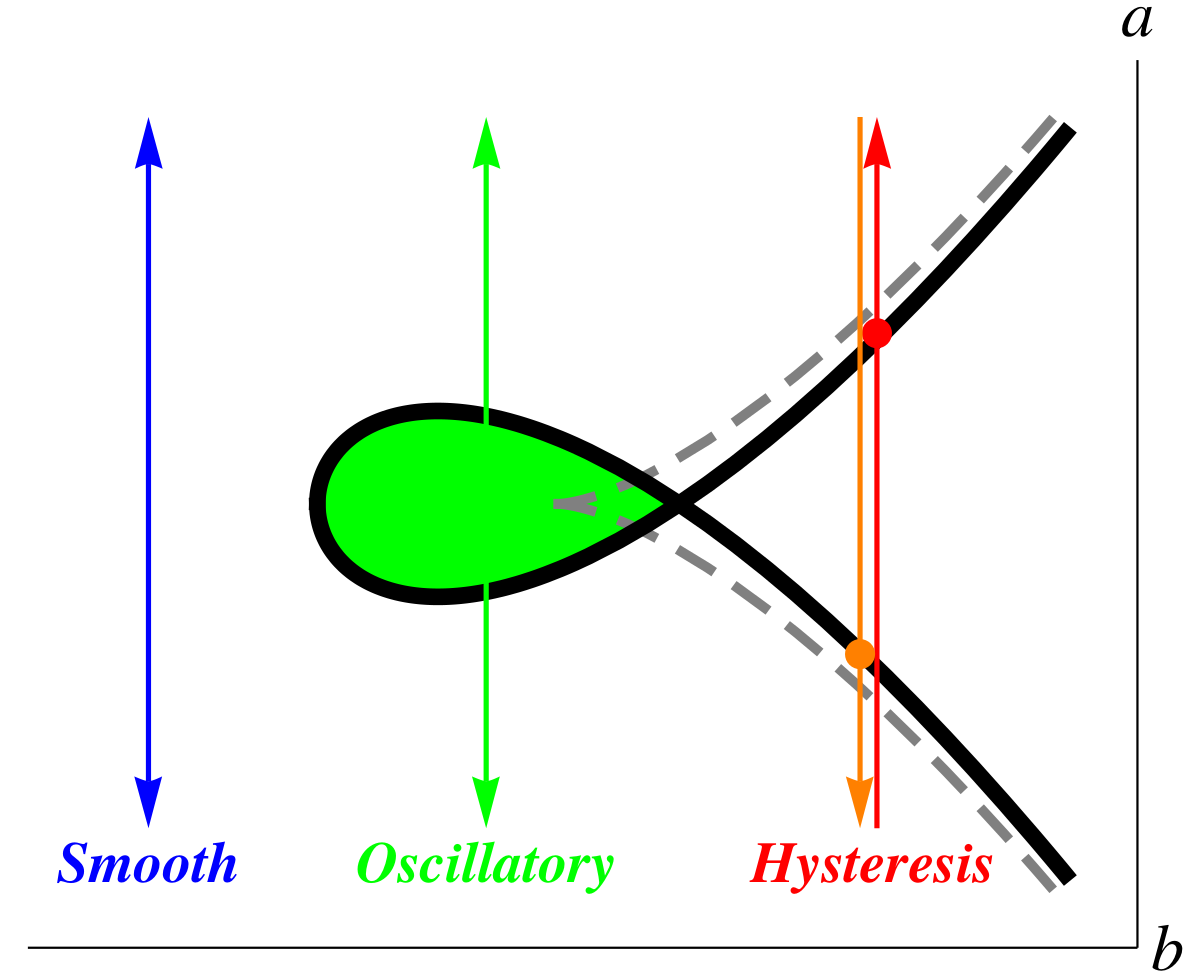
\includegraphics[width=0.9\textwidth]{../Graphics/Bif_Graphs/3_transitions_single_simple.png}
\end{minipage}
\hfill
\begin{minipage}{0.49\linewidth}
	\caption{A parameter plot of the FitzHugh-Nagumo model (Equations \ref{eq:FitzHugh-Nagumo}), a co-dimension 3 bifurcation with the black line indicating the fold bifurcation.
	This model is the one under consideration for accurately describing the L--H transition in tokamak plasmas, with the $b$ parameter dictating the type of transition.
	This $b$ parameter is akin to the density at the edge \cite{weymiens_bifurcation_2014}.}
	\label{fig:co-3}
\end{minipage}
\end{figure}

In order to accurately model to our current knowledge, the oscillatory transition must be incorporated with the sharp and smooth transitions.
Work by Weymiens \cite{weymiens_bifurcation_2014} proves that a ``co-dimension 3 bifurcation robustly connects the three types of transition behavior'' and investigates using the FitzHugh-Nagumo model.
\begin{subequations}
\begin{align} % FitzHugh-Nagumo model
	\dot{x} \,&=\, a - bx - x^3 + cy~, \\
	\dot{y} \,&=\, -y - x~.
\end{align}
	\label{eq:FitzHugh-Nagumo}
\end{subequations}
This couples the cusp bifurcation to a damped variable, with the coupling parameter $c$.
For as long as $c$ is below some critical value, only the cusp bifurcation will be present; a large enough value gives rise to the oscillatory transition.

All three bifurcations are shown in parameter space in the right plot of Fig.~\ref{fig:co-3}, with the value of the $b$ parameter dictating the type.

\subsection{Hysteresis}\label{ssec:hysteresis}
Hysteresis is a characteristic of any system which the current state of the system depends on its history.
In physics, the most common example given is that of an external magnetic field applied to a ferromagnetic material.
When the field is removed, the material will retain some of alignment of magnetic domains, and is considered magnetized.
Of course, this property is present in many other areas of study.

As mentioned previously, the L--H transition can be characterized with hysteresis.
The threshold power for the H--L transition can be significantly lower than that of the L--H transition, leading to a region in which there is a non-unique solution to the plasma state.
This requires two separate fold bifurcations each to govern the L--H and H--L transitions separately, which, in turn, requires two types of bifurcation parameters.
The first dictates hysteresis being present in the system; varying this allows for the disappearance of hysteresis when the aforementioned two fold bifurcations merge into a cusp bifurcation.
Varying the second parameter can cause the two stable solutions to be replaced by with unstable solutions, in which the system will oscillate between the solutions.
In the FitzHugh-Nagumo model (Eq.~\ref{eq:FitzHugh-Nagumo}), these are represented by $b$ and $c$, respectively.

\section{Mechanisms}\label{sec:mechanics}
Physically, the L--H transition is a bifurcation in the turbulent transport at the edge of the tokamak.
The prevailing hypothesis for the overarching mechanism for H--mode that can be directly manipulated is that high auxiliary power develops strong sheared plasma flow and suppresses transport \cite{freidberg_plasma_2007}.

\subsection{Turbulence and Flow Shear Suppression}\label{ssec:turbulence_sheared}
Turbulence is primarily driven by the gradients of the temperature and density, which increase under higher heating.
Drift waves are considered to be the only type of turbulence that pushes radial particle flux; therefore, it dictates the severity of turbulence and linked transport at the edge of the plasma.
Particular well-known instabilities can be coupled to the drift-wave turbulence, such as the drift resistant ballooning mode, among others \cite{scott_three-dimensional_1997}.
Therefore, a form for the turbulence level will be restricted to one that adheres to the drift wave.

The turbulence $\mathcal{E}$ evolves as the following, in the absence of shear in the plasma flow
\begin{align} % Turbulence ODE
	\frac{\partial\mathcal{E}}{\partial t} \,=\, \gamma_L\mathcal{E} - \alpha_\text{sat}\mathcal{E}^2~.
	\label{eq:turbulence_ode}
\end{align}
This is the result from assuming the particle diffusivity increases linearly with the level of turbulence up to some maximum \cite{diamond_dynamics_1995}.
The first term on the right-hand side is a linear growth term, with $\gamma_L$ as the growth rate.
The second term is a nonlinear saturation term, with $\alpha_\text{sat}$ as the saturation rate.
The maximum turbulence is the ratio of the linear growth rate to the saturation rate.

It is now accepted that turbulent transport at the edge is particularly suppressed by shear in the flow of the (radial) $\mathbf{E}\times\mathbf{B}$ drift \cite{terry_suppression_2000}.
The shear stress dissociates smaller turbulent structures, with their energy and momenta transferred to larger flows.
This flow shear can be modeled as a ratio of the electromagnetic fields given by \cite{staps_backstepping_2017}
\begin{align} % Shear velocity
	\frac{\partial V_{\mathbf{E}\times\mathbf{B}}}{\partial x} \,=\, \frac{\partial}{\partial x} \left(\frac{E_r}{B}\right) \,\approx\, \frac{1}{B_\phi} \frac{\partial E_r}{\partial x}~.
	\label{eq:velocity_shear}
\end{align}
Both zonal and mean $\mathbf{E}\times\mathbf{B}$ flows are responsible for the drift-wave turbulence.
Zonal flows in particular are present in L--mode, in which the shear due to Reynolds stress comes from radial and poloidal perturbations \cite{diamond_zonal_2005}.
However, they disappear in H--mode, leaving only mean flows present.

The flow shear could reduce the growth rate of the turbulence \cite{diamond_self-regulating_1994}, which was coined the linear model.
The other possibility is that flow shear can increase the saturation mechanism, which is the nonlinear model \cite{hahm_rotation_1994}.
Each are implemented as some parameter that multiplies against their respective term in Equation~\ref{eq:turbulence_ode}.
For example, the nonlinear model would adjust it to the following
\begin{align} % Nonlinear Turbulence ODE
	\frac{\partial\mathcal{E}}{\partial t} \,=\, \gamma_L\mathcal{E} - \eta_\text{NL}\alpha_\text{sat}\mathcal{E}^2~, ~~~~
	\eta_\text{NL} \,=\, 1 + \tilde{\eta} \left|\frac{\partial V_{\mathbf{E}\times\mathbf{B}}}{\partial x}\right|^2.
	\label{eq:nonlinear_turbulence_ode}
\end{align}
Both forms were investigated by Weymiens, and the nonlinear model proved more robust to changes in plasma parameters \cite{weymiens_bifurcation_2014}.
Therefore, this nonlinear model will be used in this study.

In slab geometry, a radial electric field is proportional to $V_{\mathbf{E}\times\mathbf{B}}$, allowing us to substitute in $Z$, a normalized form of the radial electric field.
The details of $Z$ are described in the following section \ref{ssec:E_r}.
This changes the coefficient of the nonlinear turbulence model $\eta_\text{NL}$ into
\begin{align} % New Saturation Coefficient
	\eta_\text{NL} \,=\, 1 + \tilde{\eta} \left|\frac{\partial V_{\mathbf{E}\times\mathbf{B}}}{\partial x}\right|^2
	\,=\, 1 + \eta\left|\frac{\partial Z}{\partial x}\right|^2~,
	\label{eq:saturation_normalization}
\end{align}
with $\eta$ including the normalization.

\subsection{Radial Electric Field}\label{ssec:E_r}
To generate a poloidal $\mathbf{E}\times\mathbf{B}$ flow with a mainly toroidal $\mathbf{B}$, an electric field must be generated.
A plethora of individual processes for the generation of such an electric field have been proposed, most of which can be viewed as separate contributions in a radial Poisson's law, with some that tend to reduce the field.
The radial electric field $E_r$ can be deduced from the radial force balance in steady-state for any plasma species $j$, as follows:
\begin{equation}
	E_r \,=\, -\frac{1}{n_j e_j} \frac{\text{d} p_j}{\text{d} r} + V_{\theta j} B_\phi - V_{\phi j} B_\theta
	\label{eq:E_r}
\end{equation}
In the above, $e_j$ represents the charge of the $j$-th species, $n_j$ is the density, $p_j$ is the pressure, and $V_{\theta j}$ and $V_{\phi j}$ are the poloidal and toroidal velocities, respectively.
This grants changes in the radial electric field to be associated with changes in radial gradient of the pressure or either velocities \cite{connor_review_2000}.
Experimentally, each term can be measured separately; however, determining these values is difficult due to large possible error.

As alluded to in the previous section, a definition of the normalized radial electric field is needed.
The definition used is
\begin{align} % Z definition
	Z \,\equiv\, \frac{\rho_p e E_r}{T}~, ~~~~ \rho_p \,\equiv\, \frac{m_i v_\text{th}}{e B_\theta}~,\label{eq:Z_and_rho_definitions}
\end{align}
with the ion mass $m_i$, the thermal ion velocity $v_\text{th}$, the elementary charge $e$, and the poloidal magnetic field $B_\theta$.

Rather than looking at an overall effect, an alternate method to determine the electric field is to look for the sources.
This means investigating the particle fluxes that go across the magnetic flux surfaces.
Any radial fluxes can be categorized as ambipolar or nonambipolar.
Ambipolar fluxes have an equal effect on electrons and all species of ions, resulting in no overall radial current.
Nonambipolar fluxes affect various charged particles differently, and thus create an electric field.
This resulting field creates a return current so that the divergence of the plasma current, on average, returns to zero.
The evolution of the field is determined by the sum of all possible radial currents, with $\Gamma_j$ referring to only nonambipolar fluxes of species $j$, since those are the ones to contribute to the field.
\begin{align} % Ambipolarity constraint
	\epsilon_0 \frac{\partial E_r}{\partial t} \,=\, -\sum J_r \,=\, \sum_j q_j\Gamma_j
	\label{eq:ambipolarity_constraint}
\end{align}

Kinetic and atomic processes contribute to the nonambipolar fluxes, in addition to fluid processes implied by the description.
These include ion orbit loss and charge exchange friction.
Details on the nonambipolar fluxes utilized in this investigation are described in depth in Section~\ref{sec:nonambipolar_fluxes}.

\section{Research Questions}\label{sec:research_questions}
Although there have been compilations of different theories describing the transition, there is yet to be a conclusive, comprehensive one \cite{connor_review_2000}.
There is substantial evidence, both theoretically and experimentally, that a radial electric field is an integral piece in the forming and enforcing of H--mode.
Many of the effects in generating and suppressing the field show up as additive terms in an equation for a radial displacement current.
Because many of these fluxes scale differently, simple scaling laws for H--mode could contrast for regimes where different effects dominate.
It is therefore important to evaluate which terms dominate in their respective regimes before inquiring about global scalings.
The overall problem is thus stated simply: \textbf{Which electric field-generating terms are dominant in concrete experimental tokamak conditions?}
This is in an effort to determine which measurable and controllable values can predict H--mode.

The first consideration is to decide \textbf{which terms should be considered for investigation}, as not all nonambipolar fluxes will significantly contribute to the transition.
For example, the nonambipolar flux due to magnetic ripple loss highly depends on collisionality, in which lower collisionality results in a low flux \cite{stringer_effect_1972}.
Since a relatively ideal operation (temperature on the order of 1 keV at the edge) will be investigated, this flux can be neglected.

\textbf{Identifying what optimal form and relative strengths of each flux and subsequently implementing them} appropriately is the crucial next step.
Because the model is highly nonlinear, it is sensitive to the forms and relative strengths.
The calculation is done with a finite volume method solver, in which the results requires verification with the literature.

The main input heating power regime previously investigate was strictly limited to near the H--L transition \cite{staps_backstepping_2017}.
Performing a scan of input heating power significantly above the lower threshold could show a difference in behavior of the fluxes and resulting field.
Therefore, \textbf{what is the variation in dominance of each field-generating term across increasing input power}, including those inside and outside the regime with non-unique operational modes?



\cleardoublepage

\chapter{Bifurcation Theory and Physics of Confinement}\label{chapter:physics_bifurcation}

\section{Bifurcation Theory}\label{sec:bif_theory}
The aforementioned transitions show clear evidence of bifurcations in the plasma system.
%A defining feature of L--H transitions is that they can occur very suddenly (the so-called sharp transition), which is characteristic of fold bifurcation behavior.
Mathematically, a bifurcation is defined to be a topological or qualitative change in a system when a small and smooth change of a parameter is made.
A simple example for a fold bifurcation is the following, with $a$ representing the parameter:
\begin{equation} % Simplest fold bifurcation
	\frac{\text{d}x}{\text{d}t} \,=\, \dot{x} \,=\, a + x^2.
	\label{eq:simple_fold}
\end{equation}
This equation can behave in one of three manners:
If $a > 0$, there are no real points of equilibrium, also known as steady-state solutions.
For $a = 0$, there is one equilibrium point at $x = 0$, and two for $a < 0$, at $x = \pm\sqrt{-a}$.
Varying $a$ from some positive real number to some negative number, the fundamental behavior of the solutions changes drastically at $a = 0$ with the sudden appearance of a steady-state solution.
Equation~\ref{eq:simple_fold} is the simplest known form of a fold bifurcation, also known as the saddle-node bifurcation.
The simplest form for any dynamical system is known as the topological norm form.
A parameter plot of $x$ versus $a$ in Fig.~\ref{fig:simple_fold} illustrates this, with the green and red curves representing the stable and unstable steady-state solutions, respectively.

%{{{ Two figures for simple bifurcations (co-dimension 1 and 2)
\TwoFig{../Graphics/Bif_Graphs/Simple_fold.png}
	{Plot of parameter space for $\dot{x} = a + x^2$ (Eq.~\ref{eq:simple_fold}), with the co-dimension 1 bifurcation occurring at $a = 0$. %
	For $a < 0$, the system has two steady-state solutions; the green is stable, while the red is unstable.
	For $a > 0$, there is no steady-state solution.}
	{fig:simple_fold}
	{../Graphics/Bif_Graphs/co-2_fold.png}
	{Plot of parameter space for $\dot{x} = -(a + x - x^3)$ (Eq.~\ref{eq:sharp_bif}). %
	This system showcases two fold bifurcations (each of co-dimension 1), at the turning points $a_{\pm\text{crit}}$, with two stable regions, in green and blue. %
	The red region is an intermediate that is unstable.}
	{fig:co-2_fold}
%}}}

The co-dimension of a system refers to the lowest number of parameters required to produce the topological norm form.
Put differently, it is the number of parameters that must be varied for the bifurcation to occur.
In the case of Eq.~\ref{eq:simple_fold}, there is only a single parameter, and is thus referred to as a co-dimension 1 bifurcation \cite{weymiens_bifurcation_2014}.

\subsection{Sharp and Smooth Transition Bifurcations}
%{{{ Two figures for zeros of the co-dimension 2 bifurcation
\TwoFigOneCap{../Graphics/Bif_Graphs/stationary_b-0_8.png}
	{../Graphics/Bif_Graphs/stationary_b_1_1.png}
	{Phase plots for Eq.~\ref{eq:sharp_bif}, with different values of $a$ within each plot. %
	There is a variance in the number of zeros based on the values of $a$ in the right plot, while there is strictly one zero for all values of $a$ in the left plot. %
	When there is multiple roots, the middle zero is always unstable.}
	{fig:stationaries_b}
%}}}

The dynamic behavior of the L--H transition correspond very closely to a few certain bifurcations.
Sharp and smooth transitions are features of the cusp bifurcation.
The topological norm form of this behavior is
\begin{equation}
	\dot{x} \,=\, -(a + bx - x^3)~.
	\label{eq:sharp_bif}
\end{equation}
Figure~\ref{fig:co-2_fold} is a plot of the parameter space, indicating the stable and unstable steady-state solutions.
This cusp bifurcation can also be regarded as two co-dimension 1 folds, if one views the positive and negative $x$-domains as separate co-dimension 1 bifurcations.
The distinction between sharp and smooth transitions in this co-dimension 2 bifurcation is solely based on the $b$ parameter, shown in the plots of Figure~\ref{fig:Bif_hysteresis}.
As $b$ approaches zero from some positive value, the size of the hysteresis shrinks, with it vanishing at $b = 0$, in which the smooth transition occurs.

%{{{ Two figures for co-dimension 2 bifurcation, with surface plot
\TwoFigOneCap{../Graphics/Bif_Graphs/co-2_fold_b_var.png}
	{../Graphics/Bif_Graphs/Bif_3D.png}
	{These plots show the mentioned co-dimension 2 cusp bifurcation, composed of two co-dimension 1 fold bifurcations, as described by Equation~\ref{eq:sharp_bif}.
	The plot on the left shows cross-sections for different $b$ values, with the sharp-smooth boundary occuring at $b = 0$.
	The plot on the right is the surface plot of this same model \cite{weymiens_bifurcation_2014}.}
	{fig:Bif_hysteresis}
%}}}

\subsection{Oscillatory Transition Bifurcation}
The third type of transition dynamics in tokamak plasmas is oscillatory, in which the system rapidly oscillates between the two different modes \cite{ryter_survey_2013, zohm_mhd_1995}.
This phenomenon is referred to by various names, including dithering, I--mode, predator--prey oscillations, and limit cycle oscillations.
It is the most enigmatic of the three discussed, as the least is known about it, and requires a more-complex model than Eq.~\ref{eq:sharp_bif}.

The Hopf, also known as a Poincar\'e-Andronov-Hopf, bifurcation is another co-dimension 1 bifurcation which can describe the oscillatory transition.
It occurs when a periodic solution or limit cycle that surrounds an equilibrium point arises or disappears, when varying the parameter.
Specifically, it occurs where the real part of complex conjugated eigenvalues vanish \cite{munoz-alicea_introduction_2011}.
%{{{ Hopf Bif example and sub/super critical explanation
%When a stable limit cycle encloses an unstable equilibrium point, it is denoted as supercritical.
%For an unstable limit cycle enclosing a stable equilibrium point, it is denoted subcritical.
%The norm form of the bifurcation is as follows,
%\begin{align} % Hopf bifurcation
%	\dot{x} \,=\, x\left((\lambda + i) + b|x|^2\right)~,
%	\label{eq:hopf_bif}
%\end{align}
%with $x$ and $b$ as complex-valued.
%Consider the following polar system, with $a$ as the parameter
%\begin{subequations}
%\begin{align} % Hopf example
%	\dot{r} \,&=\, a r - r^3~, \\
%	\dot{\theta} \,&=\, -1
%\end{align}
%\end{subequations}
%}}}

\subsection{Co-dimension 3 Bifurcation}
\begin{figure}[tb] % Co-dimension 3 bifurcation cross-section
\begin{minipage}{0.49\linewidth}
	\centering
	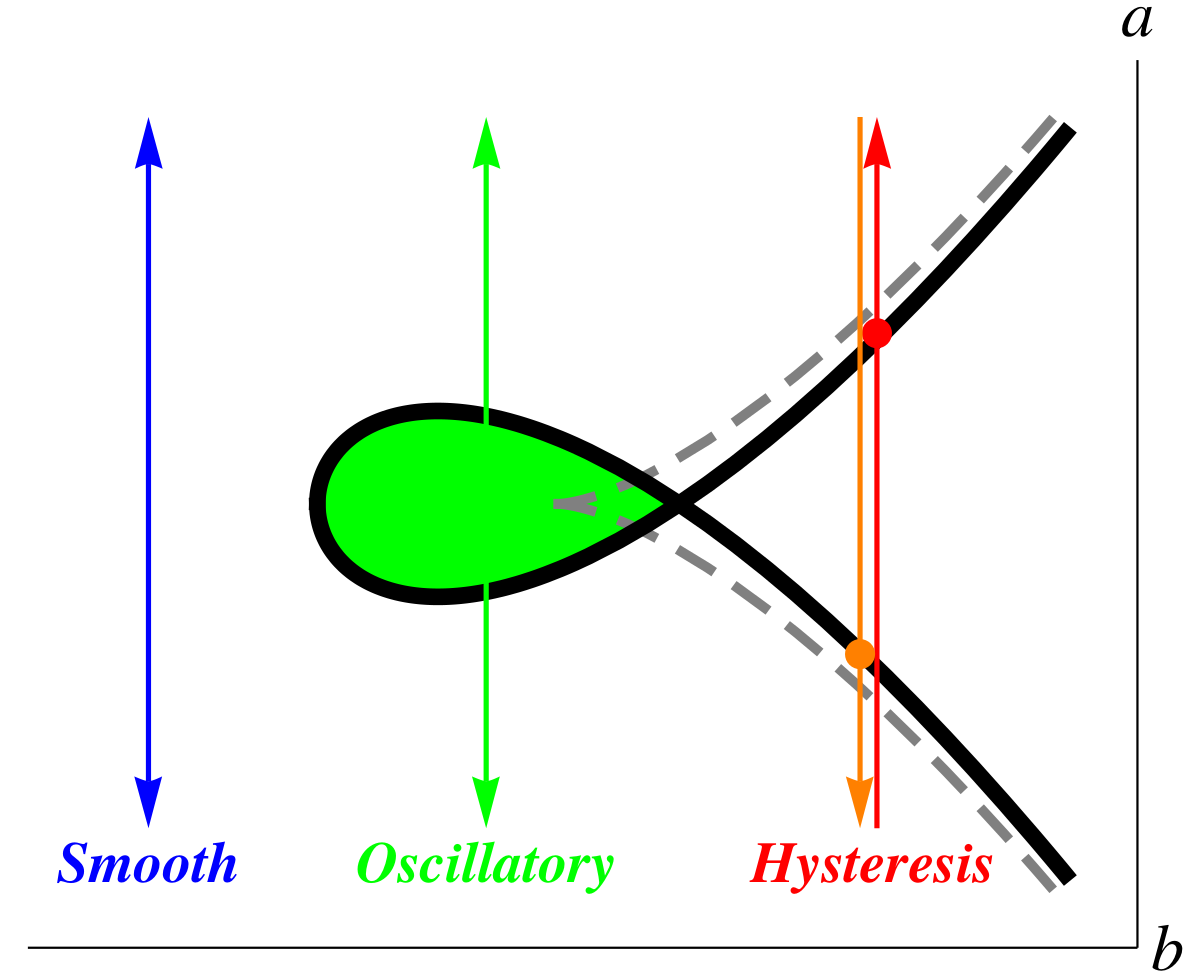
\includegraphics[width=0.9\textwidth]{../Graphics/Bif_Graphs/3_transitions_single_simple.png}
\end{minipage}
\hfill
\begin{minipage}{0.49\linewidth}
	\caption{A parameter plot of the FitzHugh-Nagumo model (Equations \ref{eq:FitzHugh-Nagumo}), a co-dimension 3 bifurcation with the black line indicating the fold bifurcation.
	This model is the one under consideration for accurately describing the L--H transition in tokamak plasmas, with the $b$ parameter dictating the type of transition.
	This $b$ parameter is akin to the density at the edge \cite{weymiens_bifurcation_2014}.}
	\label{fig:co-3}
\end{minipage}
\end{figure}

In order to accurately model to our current knowledge, the oscillatory transition must be incorporated with the sharp and smooth transitions.
Work by Weymiens \cite{weymiens_bifurcation_2014} proves that a ``co-dimension 3 bifurcation robustly connects the three types of transition behavior'' and investigates using the FitzHugh-Nagumo model.
\begin{subequations}
\begin{align} % FitzHugh-Nagumo model
	\dot{x} \,&=\, a - bx - x^3 + cy~, \\
	\dot{y} \,&=\, -y - x~.
\end{align}
	\label{eq:FitzHugh-Nagumo}
\end{subequations}
This couples the cusp bifurcation to a damped variable, with the coupling parameter $c$.
For as long as $c$ is below some critical value, only the cusp bifurcation will be present; a large enough value gives rise to the oscillatory transition.

All three bifurcations are shown in parameter space in the right plot of Fig.~\ref{fig:co-3}, with the value of the $b$ parameter dictating the type.

\subsection{Hysteresis}\label{ssec:hysteresis}
Hysteresis is a characteristic of any system which the current state of the system depends on its history.
In physics, the most common example given is that of an external magnetic field applied to a ferromagnetic material.
When the field is removed, the material will retain some of alignment of magnetic domains, and is considered magnetized.
Of course, this property is present in many other areas of study.

As mentioned previously, the L--H transition can be characterized with hysteresis.
The threshold power for the H--L transition can be significantly lower than that of the L--H transition, leading to a region in which there is a non-unique solution to the plasma state.
This requires two separate fold bifurcations each to govern the L--H and H--L transitions separately, which, in turn, requires two types of bifurcation parameters.
The first dictates hysteresis being present in the system; varying this allows for the disappearance of hysteresis when the aforementioned two fold bifurcations merge into a cusp bifurcation.
Varying the second parameter can cause the two stable solutions to be replaced by with unstable solutions, in which the system will oscillate between the solutions.
In the FitzHugh-Nagumo model (Eq.~\ref{eq:FitzHugh-Nagumo}), these are represented by $b$ and $c$, respectively.


\section{Mechanisms}\label{sec:mechanics}
Physically, the L--H transition is a bifurcation in the turbulent transport at the edge of the tokamak.
The prevailing hypothesis for the overarching mechanism for H--mode that can be directly manipulated is that high auxiliary power develops strong sheared plasma flow and suppresses transport \cite{freidberg_plasma_2007}.

\subsection{Turbulence and Flow Shear Suppression}\label{ssec:turbulence_sheared}
Turbulence is primarily driven by the gradients of the temperature and density, which increase under higher heating.
Drift waves are considered to be the only type of turbulence that pushes radial particle flux; therefore, it dictates the severity of turbulence and linked transport at the edge of the plasma.
Particular well-known instabilities can be coupled to the drift-wave turbulence, such as the drift resistant ballooning mode, among others \cite{scott_three-dimensional_1997}.
Therefore, a form for the turbulence level will be restricted to one that adheres to the drift wave.

The turbulence $\mathcal{E}$ evolves as the following, in the absence of shear in the plasma flow
\begin{align} % Turbulence ODE
	\frac{\partial\mathcal{E}}{\partial t} \,=\, \gamma_L\mathcal{E} - \alpha_\text{sat}\mathcal{E}^2~.
	\label{eq:turbulence_ode}
\end{align}
This is the result from assuming the particle diffusivity increases linearly with the level of turbulence up to some maximum \cite{diamond_dynamics_1995}.
The first term on the right-hand side is a linear growth term, with $\gamma_L$ as the growth rate.
The second term is a nonlinear saturation term, with $\alpha_\text{sat}$ as the saturation rate.
The maximum turbulence is the ratio of the linear growth rate to the saturation rate.

It is now accepted that turbulent transport at the edge is particularly suppressed by shear in the flow of the (radial) $\mathbf{E}\times\mathbf{B}$ drift \cite{terry_suppression_2000}.
The shear stress dissociates smaller turbulent structures, with their energy and momenta transferred to larger flows.
This flow shear can be modeled as a ratio of the electromagnetic fields given by \cite{staps_backstepping_2017}
\begin{align} % Shear velocity
	\frac{\partial V_{\mathbf{E}\times\mathbf{B}}}{\partial x} \,=\, \frac{\partial}{\partial x}
			\left(\frac{E_r}{B}\right) \,\approx\, \frac{1}{B_\phi} \frac{\partial E_r}{\partial x}~.
	\label{eq:velocity_shear}
\end{align}
Both zonal and mean $\mathbf{E}\times\mathbf{B}$ flows are responsible for the drift-wave turbulence.
Zonal flows in particular are present in L--mode, in which the shear due to Reynolds stress comes from radial and poloidal perturbations \cite{diamond_zonal_2005}.
However, they disappear in H--mode, leaving only mean flows present.

The flow shear could reduce the growth rate of the turbulence \cite{diamond_self-regulating_1994}, which was coined the linear model.
The other possibility is that flow shear can increase the saturation mechanism, which is the nonlinear model \cite{hahm_rotation_1994}.
Each are implemented as some parameter that multiplies against their respective term in Equation~\ref{eq:turbulence_ode}.
For example, the nonlinear model would adjust it to the following
\begin{align} % Nonlinear Turbulence ODE
	\frac{\partial\mathcal{E}}{\partial t} \,=\, \gamma_L\mathcal{E} -
		\eta_\text{NL}\alpha_\text{sat}\mathcal{E}^2~, ~~~~ \eta_\text{NL} \,=\,
		1 + \tilde{\eta} \left|\frac{\partial V_{\mathbf{E}\times\mathbf{B}}}{\partial x}\right|^2.
	\label{eq:nonlinear_turbulence_ode}
\end{align}
Both forms were investigated by Weymiens, and the nonlinear model proved more robust to changes in plasma parameters \cite{weymiens_bifurcation_2014}.
Therefore, this nonlinear model will be used in this study.

In slab geometry, a radial electric field is proportional to $V_{\mathbf{E}\times\mathbf{B}}$, allowing us to substitute in $Z$, a normalized form of the radial electric field.
The details of $Z$ are described in the following section \ref{ssec:E_r}.
This changes the coefficient of the nonlinear turbulence model $\eta_\text{NL}$ into
\begin{align} % New Saturation Coefficient
	\eta_\text{NL} \,=\, 1 +
		\tilde{\eta} \left|\frac{\partial V_{\mathbf{E}\times\mathbf{B}}}{\partial x}\right|^2
		\,=\, 1 + \eta\left|\frac{\partial Z}{\partial x}\right|^2~,
	\label{eq:saturation_normalization}
\end{align}
with $\eta$ including the normalization.

\subsection{Radial Electric Field}\label{ssec:E_r}
To generate a poloidal $\mathbf{E}\times\mathbf{B}$ flow with a mainly toroidal $\mathbf{B}$, an electric field must be generated.
A plethora of individual processes for the generation of such an electric field have been proposed, most of which can be viewed as separate contributions in a radial Poisson's law, with some that tend to reduce the field.
The radial electric field $E_r$ can be deduced from the radial force balance in steady-state for any plasma species $j$, as follows:
\begin{equation} % Lorentz Force Balance
	E_r \,=\, -\frac{1}{n_j e_j} \frac{\text{d} p_j}{\text{d} r} + V_{\theta j} B_\phi - V_{\phi j} B_\theta
	\label{eq:E_r}
\end{equation}
In the above, $e_j$ represents the charge of the $j$-th species, $n_j$ is the density, $p_j$ is the pressure, and $V_{\theta j}$ and $V_{\phi j}$ are the poloidal and toroidal velocities, respectively.
This grants changes in the radial electric field to be associated with changes in radial gradient of the pressure or either velocities \cite{connor_review_2000}.
Experimentally, each term can be measured separately; however, determining these values is difficult due to large possible error.

As alluded to in the previous section, a definition of the normalized radial electric field is needed.
The definition used is
\begin{align} % Z definition
	Z \,\equiv\, \frac{\rho_\theta e E_r}{T}~, ~~~~
		\rho_\theta \,\equiv\, \frac{m_i v_\text{th}}{e B_\theta}~,\label{eq:Z_and_rho_definitions}
\end{align}
with the ion mass $m_i$, the thermal ion velocity $v_\text{th}$, the elementary charge $e$, and the poloidal magnetic field $B_\theta$.

Rather than looking at an overall effect, an alternate method to determine the electric field is to look for the sources.
This means investigating the particle fluxes that go across the magnetic flux surfaces.
Any radial fluxes can be categorized as ambipolar or nonambipolar.
Ambipolar fluxes have an equal effect on electrons and all species of ions, resulting in no overall radial current.
Nonambipolar fluxes affect various charged particles differently, and thus create an electric field.
This resulting field creates a return current so that the divergence of the plasma current, on average, returns to zero.
The evolution of the field is determined by the sum of all possible radial currents, with $\Gamma_j$ referring to only nonambipolar fluxes of species $j$, since those are the ones to contribute to the field.
\begin{align} % Ambipolarity constraint
	\epsilon_0 \frac{\partial E_r}{\partial t} \,=\, -\sum J_r \,=\, \sum_j q_j\Gamma_j
	\label{eq:ambipolarity_constraint}
\end{align}

Kinetic and atomic processes contribute to the nonambipolar fluxes, in addition to fluid processes implied by the description.
These include ion orbit loss and charge exchange friction.
Details on the nonambipolar fluxes utilized in this investigation are described in depth in Section~\ref{sec:nonambipolar_fluxes}.




\cleardoublepage

\chapter{Dynamical Model}\label{chapter:dynamical_model}
Fusion plasmas are inherently complicated systems, and thus are complicated to model, even when taking simplification liberties.
The model developed by Itoh \emph{et al.} \cite{itoh_edge_1991} and Zohm \cite{zohm_dynamic_1994}, and later refined by others, assumes that the transport barrier occurs in a thin layer at the plasma edge.
The plasma edge is defined to be at the last-closed flux surface (separatrix).
This allows for slab geometry to be used, in which $\psi$ is a usual radial coordinate.
However, $x$ will be used as it is more distinct as a spatial coordinate.
The slab geometry reduces the model into a system of one (spatial) dimensional partial differential equations.
The domain of the model is $0 \,\leq\, x \,\leq\, L$, in which $x = 0$ is the plasma outer edge, and $x = L$ is some depth towards the core.

\section{Transport Equations}\label{sec:transport_eqs}
To model the transport of a fully-ionized fusion plasma, conservation of mass and energy are considered.
These lead to continuity equations of plasma density $n$ and internal energy $U$
\begin{align} % n and U continuity
	\frac{\partial n}{\partial t} \,+\, \frac{\partial \Gamma}{\partial x} \,&=\, 0~,\label{eq:n_continuity} \\
	\frac{\partial U}{\partial t} \,+\, \frac{\partial q}{\partial x} \,&=\, 0\label{eq:U_continuity}~.
\end{align}
The particle flux $\Gamma$ is determined by some effective particle diffusion $D$ due to anomalous transport.
Note that $\Gamma$ here refers to all species of particle fluxes, both ambipolar and nonambipolar.
The heat flux $q$, however, is determined by effective heat convection.
This is the sum of heat diffusion $\chi n T^\prime$, and advection $\Gamma T$.
\begin{align} % Fluxes
	\Gamma \,&=\, -D \frac{\partial n}{\partial x}~,\label{eq:particle_flux} \\
	q \,&=\, -\chi n \frac{\partial T}{\partial x} \,+\, \frac{\Gamma T}{\gamma - 1} \label{eq:heat_flux}
\end{align}
The adiabatic index $\gamma$ will be set to $5/3$, as is customary for monatomic gases.
It is important to note that these fluxes omit explicit drift velocities as well as particle and heat sources from within the domain of the model \cite{zohm_dynamic_1994}.

The particle and heat diffusivities $D$ and $\chi$ are considered to be functions of the turbulence.
The L-H transition is not expected to be caused by a difference in form between the two diffusivities.
It is therefore assumed they are proportional
\begin{align} % chi-D relation
	\chi \,=\, \frac{D}{\zeta (\gamma - 1)} \label{eq:heat_particle_diff_relation}~.
\end{align}
The parameter $\zeta$ determines the coupling strength of the two diffusivities. The specifics of the forms chosen for the diffusivities is discussed in Section~\ref{sec:diffusivities}.

In order to simplify the model, substituting the following definition of the internal energy should be made.
\begin{align} % U definition
	U \,\equiv\, \frac{n T}{\gamma - 1} \label{eq:U_definition}
\end{align}
In addition, one of the liberties taken to simplify the model is that a single temperature is used, \emph{i.e.} the electron and ion temperatures are assumed identical.
Making this substitution, along with the particle and heat fluxes, we can arrive at relegated forms of Equations~\ref{eq:n_continuity} and \ref{eq:U_continuity}.

\begin{align} % Compact transport equations
	\frac{\partial n}{\partial t} \,&=\, \frac{\partial}{\partial x} \left[D \,
		\frac{\partial n}{\partial x}\right]~,\label{eq:n_compact} \\
	\frac{\partial(n\,T)}{\partial t} \,&=\, \frac{\partial}{\partial x}
		\left[\frac{D\,n}{\zeta} \, \frac{\partial T}{\partial x}\right]
		\,+\, \frac{\partial}{\partial x}
		\left[D\,T \, \frac{\partial n}{\partial x}\right]~. \label{eq:U_compact}
\end{align}

The product rules of the derivatives can subsequently be worked out to obtain a further-reduced form.
One convenience is that Equation~\ref{eq:n_continuity} shows up as a collection of terms within Equation \ref{eq:U_compact}.
This allows those terms to vanish:
\begin{align} % More reduced temperature equation
	\frac{\partial T}{\partial t} \,&=\, \frac{\partial}{\partial x} \left[\frac{D}{\zeta} 
		\, \frac{\partial T}{\partial x}\right] \,+\,
		\left(1 + \frac{1}{\zeta}\right) \frac{\partial n}{\partial x} \,
		\frac{\partial T}{\partial x}~. \label{eq:T_compact}
\end{align}

\section{Nonambipolar Particle Fluxes}\label{sec:nonambipolar_fluxes}
As described in Section~\ref{ssec:E_r}, the dynamics of the radial electric field will be determined by investigating the various nonambipolar fluxes.
The fluxes chosen for this analysis comes from a compilation by Callen \cite{callen_toroidal_2009}, Itoh and Itoh \cite{itoh_role_1996}, and Stringer \cite{stringer_explanation_1993}.

For added context, the profiles of these fluxes will also be given with a typical L-- and H--mode density, temperature, and $Z$ profiles, given in Figures~.

\subsection{Polarization Current}\label{ssec:polarization_current}
In Maxwell's correction of Amp\`ere's law, a polarization current is induced whenever the time derivative of an electric field is non-zero.
This originates from the changing state of polarization.
\begin{align} % Polarization current
	J_\text{pol} \,=\, \frac{m_i \, n}{\epsilon_0\,\mu_0 \, B_\theta^2} \, \frac{\partial E_r}{\partial t}
		\,=\, \frac{\sum_j m_j n_j}{B_\theta^2} \, \frac{\partial E_r}{\partial t}
		\label{eq:polarization_current_original}
\end{align}
This is larger than the classical polarization by a factor of $B^2 / B_\theta^2$ \cite{hinton_neoclassical_1984}.
\todo{\color{red}FINISH!}

\subsection{Shear Viscosity}\label{ssec:shear_viscosity}
The ion shear (perpendicular) viscosity is the perpendicular component of the viscous stress tensor.
In the L--H transition, it can be viewed as coupling the L-- and H--mode solutions spatially.
It is expressed by Itoh \emph{et al.} \cite{itoh_elmy_1993} as
\begin{align} % Shear Viscosity Current
	J^{\pi\perp} \,=\, \nabla \left(\frac{e \, \mu_i \, n \, \rho_{\theta i}}
		{v_{T_i}} \, \nabla\left(\frac{E_r}{B_\theta}\right)\right) \,=\,
		\nabla \left(\frac{m_i \, n \, \mu_i}{B_\theta^2} \, \nabla E_r\right)~.
		\label{eq:shear_visc_current_definition}
\end{align}
The ion shear viscosity coefficient $\mu_i$ is assumed to be constant over space for simplicity.
Reducing this expression to the one radial direction, and introducing the perpendicular dielectric permittivity $\epsilon_\perp$ \cite{kiviniemi_numerical_2001} gives
\begin{align} % Current with perpendicular permittivity
	J^{\pi\perp} \,=\, e\,\Gamma_i^{\pi\perp} \,&=\,
		-\epsilon_0\,\epsilon_\perp \frac{\partial}{\partial x}
		\left(\mu_i \, \frac{\partial E_r}{\partial x}\right)~, \\
	\epsilon_\perp \,&=\, 1 + \sum_j \frac{m_j \, n_j}{\epsilon_0 \, B_\theta^2}~.
		\label{eq:perp_permittivity}
\end{align}
If one assumes that $n_i \approx n_e$ and $m_i \gg m_e$, then the sum for Eq.~\ref{eq:perp_permittivity} is only the ion term and the shear viscosity current is written
\begin{align} % Definition of perpendicular permittivity
	e \, \Gamma_i^{\pi\perp} \,=\, -\frac{m_i}{B_\theta^2} \,
		\frac{\partial}{\partial x} \left(n \, \mu_i \,
		\frac{\partial E_r}{\partial x}\right)~. \label{eq:shear_current_E_r}
\end{align}

Normalizing this expression such that it is expressed in terms of $Z$ results in
\begin{align} % Final result of shear viscosity flux, normalized
	\Gamma^{\pi\perp} \,=\, \frac{m_i \, \mu_i \, n \, T}{e^2 \, \rho_{\theta i}}
		\, \frac{\partial^2 Z}{\partial x^2} \label{eq:shear_current_Z}
\end{align}
Refer to Appendix \ref{chapter:Normalization} to see the derivation.


\subsection{Bulk Viscosity}\label{ssec:bulk_viscosity}
Two mathematical forms of the parallel ion (bulk) viscosity have been developed in the literature.
Shaing \emph{et al.} \cite{shaing_bifurcation_1990} derives an expression directly for the viscosity by solving the drift kinetic equation with mass flow velocity.
\begin{align}% Shaing Bulk Viscosity
	\langle \mathbf{B}_\theta \cdot \nabla \cdot \boldsymbol{\pi} \rangle \,=\,
		\frac{\epsilon^2 \, m_i \, B \sqrt{\pi}}{4} \, \frac{n\,v_{T_i}}{x}
		\left(I_\theta U_\theta \,+\, I_\phi U_{\theta 0}\right)
		\label{eq:shaing_bulk}
\end{align}
Here, $\boldsymbol{\pi}$ is the ion viscosity tensor, and $U_\theta$ and $U_{\theta 0}$ indicate poloidal flow velocities.
The terms $I_\phi$ and $I_\theta$ represent large poloidal and toroidal integrals, respectively, which are quite taxing to compute.

However, in an effort to circumvent the direct calculations of flow velocities, a different form is used in this investigation, introduced by Stringer \cite{stringer_explanation_1993}.
\begin{align} % Stringer Bulk Viscosity
	\Gamma_i^{\pi\parallel} \,=\, \,n_e\,&D_{\pi\parallel}
		\left(\frac{n^\prime}{n} + \frac{Z}{\rho_{\theta i}}\right) \,
		\text{Im}\left[X\left(Z + i\,\frac{\nu_{ii}}{\omega_t}\right)\right]
		\label{eq:stringer_Gamma_bulk} \\
	&D_{\pi\parallel} \,=\, \frac{\epsilon^2\,\rho_{\theta i}\,T}
		{(x - a_m)\sqrt{\pi}\,B} \label{eq:stringer_D_bulk}
\end{align}
The particle diffusivity for this process is $D_{\pi\parallel}$, which is on the order of $10^{-2}$~m$^2 / $s.
The complex-valued function $X(z)$ is the plasma dispersion function.
It appears in the dispersion equation for linearized waves in a non-relativistic plasma when the velocity distribution is Maxwellian \cite{fried_plasma_2015}.
\begin{align} % Plasma Dispersion Function
	X(z) \,\equiv\, i\,\sqrt{\pi} \, e^{-z^2} \, \text{erfc}(-i\,z) \,=\,
		\frac{1}{\sqrt{\pi}} \int_{-\infty}^{+\infty} \frac{e^{-t^2}}{t - z}
		\, \text{d}t \label{eq:plasma_disp}
\end{align}
\emph{\textbf{Note}} that this function is usually denoted as $Z$, but I am breaking this standard notation to avoid ambiguity with the normalized radial electric field.

In addition, although this flux, at first glance, may take a similar shape to subsequently-presented fluxes, the plasma dispersion function does not allow for a direct comparison in the form of Eq.~\ref{eq:Gamma_an_g}.\todo{\color{red}REMOVE?}

\subsection{Electron Anomalous Diffusion}\label{ssec:an_diffusion}
Turbulence affects ions and electrons differently, which can cause a nonambipolar flux.
In particular, when a drift wave turbulence interacts with the edge of plasma, it preferentially removes electron momentum out of the confined plasma \cite{itoh_model_1988} \cite{stringer_non-ambipolar_1995}.
The particle flux for this effect can be written as
\begin{align} % Gamma_an original and D_an
	\Gamma_e^\text{an} \,=\, -n_e \, &D^\text{an} \left(\frac{n^\prime}{n} \,+\,
		\frac{\alpha_\text{an}\,T_e^\prime}{T_e} \,+\, \frac{e\,E_r}{T_e}\right)
		\label{eq:Gamma_an_orig} \\
	&D_\text{an} \,=\, \frac{\epsilon^2 \sqrt{\pi}}{2 a_m}
		\frac{\rho_{\theta e} \, T_e}{B} \label{eq:D_an}
\end{align}
The numerical constant $\alpha_\text{an}$ is on the order of unity, and $D_\text{an}$ is the diffusion coefficient for this process.
We can normalize the electric field, rewrite the terms with `gradient' coefficients $g_l^\text{k}$ for coefficient $l$ and mechanism $\text{k}$.
\begin{align} % Gamma_an g's
	e\,\Gamma_e^\text{an} \,&=\, g_n^\text{an}\,\frac{n^\prime}{n} \,+\,
		g_T^\text{an}\,\frac{T^\prime}{T} \,+\,
		g_Z^\text{an}\,Z \label{eq:Gamma_an_g} \\
	g_n^\text{an} \,=\, -e \, n \, &D_\text{an}~,~~~~
		g_T^\text{an} \,=\, \alpha_\text{an} \, g_n^\text{an}~,~~~~
		g_Z^\text{an} \,=\, \frac{g_n^\text{an}}{\rho_{\theta i}}
		\label{eq:g_an}
\end{align}

\subsection{Charge Exchange Friction}\label{ssec:cx_friction}
With toroidal rotation, the charge exchange process between ions and neutrals causes a momentum imbalance for the charged plasma, as the momentum goes to the neutrals.
This momentum loss causes a charge imbalance, leading to a current \cite{toda_theoretical_1997}.

The charge exchange rate is obtained from a qualitative scheme by Connor and Wilson \cite{connor_review_2000}, in which the ``weak function'' $\phi_\text{cx}$ is an exponential decay.
\begin{align} % Charge exchange rate
	\langle \sigma_\text{cx} v\rangle \,=\, \frac{C_\text{cx}}{\sqrt{T}} \,
		\exp\left[-\frac{E_0}{T}\right] \label{eq:cx_rate}
\end{align}
Electrons are not exchanged above a particular temperature threshold, but rather fully ionized and lost to the bulk plasma.
The term $E_0$ is simply the ionization energy for the particular species used; hydrogen is investigated in this project, and the term is thus set to 13.6 eV.
The coefficient $C_\text{cx}$ is a numerical constant that chooses the maximum rate.

\begin{align} % Charge exchange current
	e\,\Gamma_e^\text{cx} \,&=\,
		-\frac{m_i \,n_0 \langle\sigma_\text{cx} v\rangle \, n\,T}{B_\theta^2}
		\, \left[\frac{B_\theta^2}{\epsilon^2 B_\phi^2} + 2\right] \,
		\left(\frac{n^\prime}{n} \,+\, \frac{\alpha_\text{cx}\,T^\prime}
		{T} - \frac{Z}{\rho_{\theta i}}\right) \label{eq:Gamma_cx}
\end{align}

We can write the terms in a similar fashion to Eqs.~\ref{eq:Gamma_an_g} as comparison.
\begin{align} % Charge exchange g's
	g_n^\text{cx} \,=\, -\frac{m_i \,n_0 \langle\sigma_\text{cx} v\rangle \,n T}
		{B_\theta^2}& \left[\frac{B_\theta^2}{\epsilon^2 B_\phi^2} + 2\right]
		~,~~~~ g_T^\text{cx} \,=\, \alpha^\text{cx}\,g_n^\text{cx}~,~~~~
		g_Z^\text{cx} \,=\, -\frac{g_n^\text{cx}}{\rho_{\theta i}}
		\label{eq:g_cx}
\end{align}
\todo{\color{red}FINISH}

\subsection{Ion Orbit Loss}\label{ssec:ol_loss}
The loss of ions due to each's individual orbit is a radial current that has certainly been seen in experiments \cite{weisen_boundary_1991}.
Again, due to the fact that ions are significantly more massive than electrons, the size of their gyroradius and banana orbits are significantly different.
When an ion follows a field line which is less than the distance of one gyroradius away from the last close flux surface, the ion is lost.
This current, also referred to as the ion loss cone, is compounded by the fact that it is highly affected by the electric field.
\begin{align} % Ion orbit loss definition
	\Gamma_i^\text{OL} \,=\, n \, \rho_{\theta i} \, (\nu_{ii} + \nu_{in_0})
		\sqrt{\epsilon} \, \frac{\exp\left[-\sqrt{\nu_{*i} + Z^4 +
		\left(\frac{x}{w_{bi}}\right)^4}\right]}{\sqrt{\nu_{*i} + Z^4 +
		\left(\frac{x}{w_{bi}}\right)^4}} \label{eq:Gamma_OL}
\end{align}
The term $\nu_{*i}$ is the ion-ion collision frequency upon the ion banana bounce frequency, and $\nu_{in_0}$ is the ion-neutral collision frequency.
The sum of the ion-ion and ion-neutral frequency serves as the effective detrapping frequency.
This particular form highly localizes the effect of the radial electric field \cite{kobayashi_experimental_2016}.

\section{Radial Electric Field Equation}\label{sec:Z_equation}
A rigorous theory on what causes the diffusion coefficients $D$ and $\chi$ is still unknown.
%However, experiments and mathematical investigations indicate that flows in the plasma can tear apart turbulent eddies, which reduces the transport radially.\todo{\color{red}{Reword?}}
To model the dynamics of the transition fully within this scope, the radial electric field must also be evolved explicitly.
As shown previously, the radial electric field $E_r$ is normalized with the ion poloidal gyroradius $\rho_\theta$ into $Z$ for this investigation, shown in Equation~\ref{eq:Z_and_rho_definitions}.

Itoh \emph{et al.}, originally modeled an evolution to the radial electric field, which included hysteresis and an oscillatory phase \cite{itoh_edge_1991}
\begin{align} % Original Itoh model
	\frac{\partial Z}{\partial t} \,&=\, -N(Z,g) + \mu \frac{\partial Z^2}{\partial x^2}~,\label{eq:original_z} \\
	N(Z,g) \,&\equiv\, g - g_0 + \left[\beta Z^3 - \alpha Z\right]~.
\end{align}
The nonlinear $N(Z,g)$ function introduces the bifurcating behavior, with $g$ acting as a gradient parameter, and $g_0$, $\alpha$, and $\beta$ as the bifurcation parameters \cite{itoh_model_1988}.
Weymiens \cite{weymiens_bifurcation_2012} rewrote the equation as
\begin{align} % Modern model
	\epsilon \, \frac{\partial Z}{\partial t} \,=\, \mu \, \frac{\partial^2 Z}{\partial x^2} \,+\,
		\frac{c_n T}{n^2} \, \frac{\partial n}{\partial x} \,+\,
		\frac{c_T}{n} \, \frac{\partial T}{\partial x} \,+\, G(Z)~,\label{eq:paquay_Z} \\
	G(Z) \,\equiv\, a + bZ + cZ^3 \label{eq:G_polynomial}
\end{align}
\todo{\color{red}Move and expand}

\section{Forms of Diffusivities}\label{sec:diffusivities}
Various forms of $D$ (and subsequently $\chi$) are presented in investigations with this model.
The original Itoh model has $D$ proportional to the hyperbolic tangent of the normalized radial electric field \cite{itoh_edge_1991, zohm_dynamic_1994}
\begin{align} % Itoh diffusivity
	D(Z) \,&=\, \frac{D_\text{max} + D_\text{min}}{2} +
		\frac{(D_\text{max} - D_\text{min})\tanh(Z)}{2}~. \label{eq:Itoh_diffusivity}
\end{align}

However, it is now accepted that the diffusivity must be a function of the shear of the field.
This is either due to the stabilization of linear modes, or through the reduction of turbulence amplitudes, correlation lengths, or change in phases of the fluctuations \cite{connor_review_2000}.
It was found that ``a flattened (steep) radial equilibrium gradient tends to enhance (eliminate) turbulence suppression due to the shear flow'' \cite{zhang_edge_1992}.
\begin{align} % Shear diffusivity
	D(Z^{\prime}) \,=\, \frac{D_\text{min}}{1 + c(Z^{\prime})^{\gamma}} \label{eq:shear_diffusivity}
\end{align}
Staps uses this form, with $c = 0.5$ and $\gamma = 2$ \cite{staps_backstepping_2017}.
Another form includes both the field itself and its shear \cite{paquay_studying_2012}
\begin{align} % Flow-Shear equation
	D(Z, Z^{\prime}) \,=\, D_\text{min} \,+\, \frac{D_\text{max} - D_\text{min}}{1 + a_1 Z^2 + a_2 Z \cdot Z^{\prime} + a_3 (Z^{\prime})^2} \label{eq:flow-shear}
\end{align}
\todo{\color{red}Expand more!}

\section{Boundary Conditions}\label{sec:boundary_conditions}
The set of aforementioned PDE's is evaluated in a domain that is small enough to exclude the inner (core) boundary from any possible particle and heat sources.
In this model, this boundary to the domain is $x = L$, for some positive length $L$, with the core is assumed to be at $x \gg L$.
It also requires the domain to be sufficiently large to fully-encompass the transport barrier and ignore any possible boundary effects of the barrier itself.
The outer boundary of the plasma edge is assumed to be the SOL (scrape-off layer).
This corresponds to $x = 0$.

It is assumed that the SOL is passive to particle and heat fluxes, and therefore the density and temperature profiles exponentially decay.
\begin{align} % n and T boundary conditions at SOL
	n^\prime(0) \,=\, \frac{n}{\lambda_n}~, ~~~~
		T^\prime(0) \,=\, \frac{T}{\lambda_T}~.\label{eq:nT_SOL_boundary}
\end{align}
The core side has a constant influx of particles and heat, stemming from fueling and heating.
\begin{align} % Fluxes from core
	\Gamma(L) \,&=\, \Gamma_c ~\longrightarrow~ n^\prime(L)
		\,=\, \frac{\Gamma_c}{D} \label{eq:core_particle_flux}\\
	q(L) \,&=\, q_c ~\longrightarrow~ T^\prime(L) \,=\, \frac{\zeta(
		\Gamma_c \, T - (\gamma - 1)\,q_c)}{D \, n} \label{eq:core_heat_flux}
\end{align}
There are hypothesized boundary conditions for the electric field at the core, but are not confirmed in any way.



\cleardoublepage

\chapter{Numerical Method}\label{chapter:numerical_method}
The finite volume method (FVM) is a numerical method of evaluating and representing partial differential equations.
It is sometimes, confusingly, referred to as the finite difference \emph{scheme} or the cell-centered difference scheme, the former which clashes in name with the finite difference method.
There are some characteristics it has in common with the two other well-known schemes, the finite difference method and the finite element method (FEM).

All three methods involve nodes generated on a discrete mesh.
In the FVM, the nodes are surrounded by the discrete elements called control volumes, with space variables able to be defined at the volume's centers or faces.
In solving, volume integrals that contain a divergence term are converted by the divergence theorem to surface integrals.
The terms are evaluated as fluxes at the surfaces of each control volume, and are accounted for between volumes, \emph{i.e.} conserved.
It also allows for discontinuities of the coefficients, assuming it occurs on the boundaries of the volumes.
Equations \ref{eq:shear_diffusivity} and \ref{eq:flow_shear_diffusivity} contain electric field shear term(s) to some exponent, potentially generating these discontinuities.
This makes the method popular for computational fluid dynamics, of which one could consider this investigation \cite{eymard_finite_2003}.

%%%%%%%%
%The FEM is based on the variational formulation of the problem; it is obtained by multiplying the original equation by a test function.
%The unknown variable is then approximated by some linear combination of ``shape'' functions, which then the equation in each element is integrated \cite{eymard_finite_2003}.
%%%%%%%%



\cleardoublepage

\chapter{Results}\label{chapter:results}
This chapter is broken into two sections.
The first covers any verification of the changes made to the numerical parameters of the original model of the Z equation (Eq.~\ref{eq:original_Z_equation}).
The second section shows the results of the flux version, Eq.~\ref{eq:reduced_normalized_Z_equation}.\todo{\color{red}ADD MORE!}

\section{Original Model} \label{sec:original_results}
%{{{ Two time slices in the Flow-Shear Original Model
\TwoFigOneCap{\includegraphics[width=\textwidth]{../Graphics/Model_Graphs/Original_FS_0000.png}}
	{\includegraphics[width=\textwidth]{../Graphics/Model_Graphs/Original_FS_0135.png}}
	{The left plot shows the initial conditions set forth by Eqs.~\ref{eq:n_initial}--\ref{eq:T_initial}, with the right plot at a later time.
	The diffusivity was set to the Flow-Shear model, \emph{i.e.} Eq.~\ref{eq:flow_shear_diffusivity}, with $a_1 = 0.1$, $a_2 = 0$, and $a_3 = 0.5$.
	The core particle and heat fluxes, respectively, are set to $-0.8$ and $4.0$.}
	{fig:Original_FS}
%}}}

If we look at the steady-state values of the equationladkjsf;alkdsfj\todo{\color{red}ADFADFADF}
\begin{figure}[tb] % Steady-State as a function of Z, original model
	\centering
	\begin{sagesilent}
		reset()

		var('Z')

		c_n, c_T = -1.1, -0.9
		a, b, c = 3.0/2.0, 2.0, -1.0
		Z_S = -3.0/2.0

		# At t = 0
		#0.49	0.683706980466396	1.32496145938483	-0.0206250867984561	5
		#0.51	0.691213814264995	1.33027412776876	-0.0191672209048899	5
		#0.53	0.698719562491543	1.33554223315998	-0.0177733476721204	5

		# At t = 135
		#0.49	0.610660563155032	1.30411254952973	-3.06036908428267	2.66118461102601
		#0.51	0.618549890710752	1.31299641246706	-3.05151915868033	2.66386371895
		#0.53	0.626467999984115	1.32173998954979	-3.0425333319374	2.66544015688424
		# .........
		#0.99	0.981110868143376	1.63421628926577	-1.48108678379191	0.491444796219089
		#1.01	0.999673727872353	1.64981311266731	-1.28285663026662	0.499537912103461
		#1.03	1.01660486587383	1.66401200235489	-1.09300528560897	0.513478891305364
		# .........
		#1.99	1.2435198107485	1.79762273772508	0.141694442025275	4.9908892834125
		#2.01	1.24801940647034	1.79934360213636	0.141647858350999	4.99089991282975
		#2.03	1.2525541146463	1.80107077486164	0.141626086988019	4.99090015667972

		t = (0, 135, 135, 135)
		x = (0.51, 0.51, 1.01, 2.01)
		density = (0.691213814264995, 0.618549890710752, 0.999673727872353, 1.24801940647034)
		density_grad = ((0.698719562491543 - 0.683706980466396) / 0.04,\
				(0.610660563155032 - 0.626467999984115) / 0.04,\
				(1.01660486587383 - 0.981110868143376) / 0.04,\
				(1.2525541146463 - 1.2435198107485) / 0.04)
		temperature = (1.33027412776876, 1.31299641246706, 1.64981311266731, 1.79934360213636)
		temperature_grad = ((1.33554223315998 - 1.32496145938483) / 0.04,\
				(1.32173998954979 - 1.30411254952973) / 0.04,\
				(1.66401200235489 - 1.63421628926577) / 0.04,\
				(1.80107077486164 - 1.79762273772508) / 0.04)

		colors = rainbow(len(x) + 1)

		G(Z) = a + b*(Z - Z_S) + c*(Z - Z_S)^3

		steady_state_plots = []

		for j in range(len(x)):
		    f(Z) = (c_n * temperature[j] / density[j]^2) * density_grad[j] + (c_T / density[j]) * temperature_grad[j] + G(Z)
		    steady_state_plots.append(plot(f, (Z,-3.5,1.5), ymin=-3, ymax=4,\
		    		gridlines=True, color=colors[j], axes_labels=["$Z$",""],\
		    		thickness=2.0, legend_label="$x = " +str(x[j].n(digits=3))\
		    		+"$, $t = " +str(t[j].n(digits=3))+ "$"))

		steady_state_plots.append(plot(G, (Z,-3.5,1.5), gridlines=True,\
				color=colors[-1], thickness=2.0, legend_label="$G(Z)$"))

		equation_label = text(r"$f(Z) = \frac{c_n \, T}{n^2} \, \frac{\partial n}{\partial x} \,+\, \frac{c_T}{n} \, \frac{\partial T}{\partial x} \,+\, G(Z)$",\
				(-2,-2.5), bounding_box={'boxstyle': 'round', 'fc': 'w'},\
				fontsize=16, color='black')

		combined_plots = sum(steady_state_plots) + equation_label
		combined_plots.set_aspect_ratio(0.4)
	\end{sagesilent}
	\sageplot[width=0.9\textwidth]{combined_plots}
	\caption{This plot shows the steady-state values across $Z$ at different locations in the domain, corresponding with the plots in Fig.~\ref{fig:Original_FS}.
	It assumes the concavity of the field is 
	The three locations correspond to near the edge, at the transport barrier, and half-way in the domain.}
\end{figure}

\section{Flux Model} \label{sec:flux_results}

\begin{sagesilent}
	reset()
	import scipy
	from scipy import constants

	alpha_an, alpha_cx = 1.5, 1.5
	a_m, R = 0.6670832032063168, 1.6					# Minor, major radius
	B_phi = 3.9											# Toroidal field
	B_theta = constants.mu_0 * 2.0e6 / ( 2*pi * a_m )	# Poloidal field

	aspect = a_m / R									# Aspect ratio
	q = aspect * B_phi/B_theta							# q value
\end{sagesilent}

\begin{table}[!htb] % Shows flux data for a time slice at two locations
	\centering
	\begin{tabular}{r|cccc}
	\begin{sagesilent} # At x ~ 0.002, t = 200
		# THE DATA USED IN THE NEXT TABLE
		#x	$n$	$T$	$Z$	$D$	$D_{an}$	$\Gamma_e^{an}$	$n_0$	$\langle\sigma_{cx} v\rangle$	$\Gamma_i^{cx}$	$D_{\pi\parallel}$	$\Gamma_i^{\pi\parallel}$	$\Gamma_i^{ol}$
		t = 200
		x, density, temperature, Z, Diffusivity, D_an, Gamma_an, n_0, cx_rate, Gamma_cx, D_bulk, Gamma_bulk, Gamma_ol = 0.002125, 5.35434214493223e+17, 165.427742871548, 1.47166341450206, 2.13128525822014, 0.000700479137552669, 2.30504108694339e+17, 56167794581565.9, 2.5481649909684e-13, -4.83290085496657e+16, -0.0191697028228131, -1.17180463596314e+18, -466734643459656

		v_Ti = sqrt(2.0 * constants.e * temperature / constants.m_p)
		rho_pi = constants.m_p * v_Ti / (constants.e * B_theta)

		nu_ii = 1.2 * sqrt(constants.m_e / constants.m_p)\
				* 4.2058e-11 * density / sqrt(temperature^3)
		omega_t = v_Ti / (q * R)

		g_n_cx = -constants.m_p*n_0*cx_rate*density*(temperature/constants.e)\
				/ (B_theta^2) * (B_theta^2 / (aspect*B_phi)**2)
		g_T_cx = g_n_cx * alpha_cx
		g_Z_cx = g_n_cx / rho_pi
	\end{sagesilent}
		$x = \sage{(x*1000).n(digits=4)}$ mm & $\dfrac{n^\prime}{n}$ & $\dfrac{T^\prime}{T}$ & $Z$ & Total \\
		$\dagger \, \Gamma_i^{\pi\parallel}$ & $\sage{(density * D_bulk * sqrt(pi)*exp(-Z^2)).n(digits=3)}$ & --- & $\sage{((density * D_bulk / rho_pi) * sqrt(pi)*exp(-Z^2)).n(digits=3)}$ & $\sage{Gamma_bulk.n(digits=3)}$ \\
		$\Gamma_e^\text{an}$ & $\sage{(density * D_an).n(digits=3)}$ & $\sage{(density * D_an * alpha_an).n(digits=3)}$ & $\sage{(density * D_an / rho_pi).n(digits=3)}$ & $\sage{Gamma_an.n(digits=3)}$ \\
		$\Gamma_i^\text{cx}$ & $\sage{g_n_cx.n(digits=3)}$ & $\sage{g_T_cx.n(digits=3)}$ & $\sage{g_Z_cx.n(digits=3)}$ & $\sage{Gamma_cx.n(digits=3)}$ \\
		$\Gamma_i^\text{ol}$ & --- & --- & --- & $\sage{Gamma_ol.n(digits=3)}$ \\ \hline

	\begin{sagesilent} # x ~ 0.030125, t = 200
		x, density, temperature, Z, Diffusivity, D_an, Gamma_an, n_0, cx_rate, Gamma_cx, D_bulk, Gamma_bulk, Gamma_ol = 0.030125, 1.08615114035334e+18, 221.843028685801, 1.77821178953312, 4.94743894562273, 0.00108811581270749, 6.12848344919829e+17, 1943024953.06425, 2.81018035060206e-13, -4232723648741.13, -0.0310869925862421, -1.37764340545142e+18, -1.15809327369854e-59

		# Update for new values
		v_Ti = sqrt(2.0 * constants.e * temperature / constants.m_p)
		rho_pi = constants.m_p * v_Ti / (constants.e * B_theta)

		nu_ii = 1.2 * sqrt(constants.m_e / constants.m_p)\
				* 4.2058e-11 * density / sqrt(temperature^3)
		omega_t = v_Ti / (q * R)

		g_n_cx = -constants.m_p*n_0*cx_rate*density*(temperature/constants.e)\
				/ (B_theta^2) * (B_theta^2 / (aspect*B_phi)**2)
		g_T_cx = g_n_cx * alpha_cx
		g_Z_cx = g_n_cx / rho_pi
	\end{sagesilent}

		$x = \sage{(x*1000).n(digits=4)}$ mm & & & & \\
		$\dagger \, \Gamma_i^{\pi\parallel}$ & $\sage{(density * D_bulk * sqrt(pi)*exp(-Z^2)).n(digits=3)}$ & --- & $\sage{((density * D_bulk / rho_pi) * sqrt(pi)*exp(-Z^2)).n(digits=3)}$ & $\sage{Gamma_bulk.n(digits=3)}$ \\
		$\Gamma_e^\text{an}$ & $\sage{(density * D_an).n(digits=3)}$ & $\sage{(density * D_an * alpha_an).n(digits=3)}$ & $\sage{(density * D_an / rho_pi).n(digits=3)}$ & $\sage{Gamma_an.n(digits=3)}$ \\
		$\Gamma_i^\text{cx}$ & $\sage{g_n_cx.n(digits=3)}$ & $\sage{g_T_cx.n(digits=3)}$ & $\sage{g_Z_cx.n(digits=3)}$ & $\sage{Gamma_cx.n(digits=3)}$ \\
		$\Gamma_i^\text{ol}$ & --- & --- & --- & $\sage{Gamma_ol.n(digits=3)}$
	\end{tabular}
	\caption{This table shows the values of the nonambipolar fluxes at two locations in the domain.
	The upper half comes from a region of the transition, while the lower half is close to the core of the domain, indisputably in L--mode.
	The appropriate gradient coefficients are shown in the columns, \emph{i.e.} $g_l^\text{k}$.
	Note that, since bulk viscosity $\Gamma_i^{\pi\parallel}$ has a nonlinear term in the plasma dispersion function, its gradient coefficients are not entirely comparable.
	Nevertheless, they do give an indication of the relative dominance.}
	\label{table:flux_values}
\end{table}



\cleardoublepage

\chapter{Conclusion} \label{chapter:conclusion}
\section{Discussion} \label{sec:discussion}
\begin{itemize}
	\item \textbf{Which electric field-generating mechanism is dominant among the ones presented?}
\end{itemize}

The data suggests that the ion bulk viscosity $\Gamma_i^{\pi\parallel}$ consistently has the largest effect on the field, with the anomalous electron loss $\Gamma_e^\text{an}$ as second-most.
At the low end, the ion orbit loss $\Gamma_i^\text{ol}$ becomes highly suppressed once there is a nonzero value of the electric field at the edge, and thus is effectively nonexistent in H--mode.

The charge exchange friction $\Gamma_i^\text{cx}$ is highly dependent on the neutrals density, and therefore processes that result in a higher neutrals density or a deeper penetration depth dictate its dominance.
In real-world cases, any methods of increasing the neutrals will increase this effect.
In this investigation, charge exchange friction was found to not supersede the two first mentioned.

\begin{itemize}
	\item \textbf{What are the appropriate forms of each flux for the model and what are the relative sensitivities and sources of uncertainty?}
\end{itemize}

The forms of the fluxes were taken from established literature.
Two of the source fluxes go linearly with the field $Z$, while the other two are explicitly nonlinear.
A comparison can be made with the Taylor-expanded model by associating the components of the fluxes to the parameters of the expanded model.
For example, the $g_n^\text{an}$ term from the anomalous electron loss flux is certainly contained within the $c_n$ coefficient, as they are both considered coefficients to the density gradient.
Following this logic, only the bulk viscosity $\Gamma_i^{\pi\parallel}$ and ion orbit loss $\Gamma_i^\text{ol}$ can have components related to the cubic coefficient $c$ within the polynomial $G(Z)$.

The shear viscosity $\Gamma_i^{\pi\perp}$ is sensitive only to the dynamic viscosity $\mu$, and is completely necessary to have the system.
However, the charge exchange friction and anomalous electron loss both significantly depend on the density and temperature gradients, with the form of bulk viscosity used here also depending on the density gradient.
Real-world calculation of these fluxes become more difficult since error in measurements of the gradients are usually high.

The transport barrier typically forms a centimeter or two into the plasma, relatively distant from the area which the ion orbit loss is present.
Uncertainties in the position or value of $Z$ highly affect this term, but does not manifest in any significant change in $Z$ itself.
This follows exactly the behavior one would expect from $\Gamma_i^\text{ol}$.

The parameters of the diffusivity are extremely sensitive, as a small change to the coefficient of the shear viscosity $a_3$ can change the fundamental behavior of the entire system.
Due to this being a qualitative model, in which the parameters are chosen rather than calculated, the ease of the formation of the transport barrier must be tuned carefully.
Values for these parameters were found to work in these conditions, but could be the culprit of unexpected behavior.

\begin{itemize}
	\item \textbf{What is the variation in dominance of each field-generating mechanism across increasing input power?}
\end{itemize}

As of now, charge exchange friction is directly proportional to the core particle flux $\Gamma_c$, giving it quite literally a direct relation to the input power on initialization.
Unsurprisingly, ion orbit loss is least affected by input heat and particle flux from the core, as any rise to $Z$ quickly vanishes the term.
The bulk viscosity $\Gamma_i^{\pi\parallel}$ seems to be more heavily affected, potentially giving rise to unphysical oscillations.
For large enough core particle fluxes, a transport barrier can be formed, as suggested from experiment.
Excluding the bulk viscosity seems to prevent the formation.
However, the presence of a transport barrier necessitates a relatively large difference in $Z$, to which the bulk viscosity is easily suppressed.
From this, one can conclude that, within the mathematical model presented here, the bulk viscosity is the culprit for the L--H transition.

\section{Outlook} \label{sec:outlook}
A more-complete picture of the radial electric field at the edge of the plasma, and its effects, seem to be necessary in understanding the physics of H--mode and the L--H transition.
H--mode is considered necessary for viable fusion energy, and in knowing its physical origin and manner of control gives substantial progress to the field.

Due to the presence of unnatural results in this study, many of the nonambipolar fluxes may need adjustment or contextual comparison.
A more-robust form of the charge exchange friction presented here should be established and updated, both in parameters and overall form.
Since the neutrals profile takes a somewhat qualitative approach that is weakly dynamic, i.e., $k$ and $d$ are simple constants, this can only be used as a starting point.
In addition, it does not take in to account of different species of neutrals, making the flux overall too simple.
A comparison of the two bulk viscosity models is also required, with some manner of experimental verification.
The form dealt with here (Eq.~\ref{eq:stringer_Gamma_bulk}) is shown to dominate over the other fluxes; whether the alternate (Eq.~\ref{eq:shaing_bulk}) gives rise to the same effects and relative size to other nonambipolar fluxes remains to be seen.

In addition, bifurcation analysis is required to prove that the sum of the nonambipolar fluxes provides the same bifurcating behavior as the Taylor-expanded model.
If it does not, alternative forms of the nonambipolar fluxes must be implemented, and derived if needed.
Both dithering (I-) mode and hysteresis were not conclusively found in this investigation for the fluxes provided, and is needed to be investigated more deeply.
Any newly-included mechanisms, such as Reynolds stress, should be subject to this same rigor.



\cleardoublepage

% ---------------------------------------------------------

\begin{appendices}
\setcounter{tocdepth}{0}
\chapter{Plasma and Machine Parameters}\label{chapter:Plasma_Parameters}
To tie this investigation to a physical machine, ASDEX-Upgrade was chosen.
Future investigations are aided by this since a wealth of L--H transition data exists for the machine.
All temperatures are in units of eV, unless otherwise noted, and the subscript $j$ indicates either electrons or ions.

The size of the machine is as following, with $a_v = 0.8$ and $a_h = 0.5$ as the vertical and horizontal minor radii, respectively.
\begin{sagesilent}
	reset()
	load("../Sage_Model/parameters.sage")
\end{sagesilent}
\begin{align} % Physical size
	a_m \,&=\, \sqrt{\frac{a_v^2 + a_h^2}{2}} \,\approx\,
		\sage{a_m.n(digits=3)}~\text{m}~,~~~~
		R \,=\, \sage{R.n(digits=3)}~\text{m} \\
		\epsilon \,&=\, \frac{a_m}{R} \,\approx\, \sage{epsilon.n(digits=2)}
\end{align}
Note that the symbol used for the aspect ratio is $\epsilon$ without subscript.
Any value of permittivity is indicated by an $\epsilon$ \emph{with} a subscript.

The magnetic field is produced by both the toroidal coils and the central solenoid.
\begin{align} % Magnetic fields
	I_\phi \,&=\, \sage{(I_phi/1.0e6).n(digits=3)}~\text{MA}~,~~~~
		B_\theta \,=\, \frac{\mu_0 \, I_\phi}{2\pi \, a_m} \,\approx\,
		\sage{B_theta.n(digits=3)}~\text{T}, \\
	B \,&=\, \sage{B.n(digits=4)}~\text{T}
\end{align}
These allow for the calculation of the safety factor.
\begin{align} % Safety factor
	q \,=\, \frac{a_m \, B_\phi}{R \, B_\theta} \,=\,
		\frac{\epsilon \, B_\phi}{B_\theta} \,\approx\, \sage{q.n(digits=3)}
		\label{eq:safety_factor}
\end{align}

The thermal velocity is chosen as the one that selects the most probable speed.
Without affecting the outcome of the study, one could choose another scheme, as they only differ by a relatively small factor.
\begin{align} % Thermal velocity
	v_{T_j} \,=\, \sqrt{\frac{2 \, e \, T}{m_j}}
		\label{eq:thermal_velocity}
\end{align}
The frequency by which ions go from being in trapped orbits to untrapped orbits is the ion transition angular frequency.
\begin{align} % Transition frequency
	\omega_t \,=\, \frac{v_{T_i}}{q \, R} \label{eq:transition_freq}
\end{align}
The frequency by which ions/electrons ``bounce'' from one end of it's banana orbit to the other and back is the banana orbit bounce frequency.
\begin{align} % Banana frequency
	\omega_{bj} \,=\, \frac{\epsilon^{3/2} \, v_{T_j}}{q \, R}
		\label{eq:banana_bounce_freq}
\end{align}
The width of the ion banana orbit plays a crucial role in the ion orbit loss flux.
It heavily affects the penetration depth of this flux.
\begin{align} % Banana width
	w_{bi} \,=\, \rho_{\theta i} \sqrt{\epsilon} \label{eq:banana_width}
\end{align}
Electron-ion and ion-ion collision frequencies are taken from Freidberg \cite{freidberg_plasma_2007}.
\begin{align} % Electron-ion and ion-ion collision frequencies
	\nu_{ei} \,=\, 1.33\times 10^5 \, \frac{n_{20}}{(T_\text{keV})^{3/2}}
		\,&=\, 4.2058\times 10^{-5} \, \frac{n}{(T_\text{eV})^{3/2}}
		\label{eq:nu_ei} \\
	\nu_{ii} \,=\, 1.2 \, \nu_{ei} \sqrt{\frac{m_e}{m_i}} \,&=\,
		\sage{(4.2058e-5* 1.2 * sqrt(constants.m_e / constants.m_p)).n(digits=4)}
		\, \frac{n}{(T_\text{eV})^{3/2}} \label{eq:nu_ii}
\end{align}
The ion collisionality is defined as the ratio of the ion-ion collision frequency to the banana orbit frequency.
\begin{align} % Ion collisionality
	\nu_{*i} \,=\, \frac{\nu_{ii}}{\omega_{bi}} \label{eq:collisionality}
\end{align}

%\inputminted[firstline=24, lastline=33, tabsize=4, breaklines=true, fontsize=\footnotesize, frame=single, linenos=true]{python}{../FiPy_Model/parameters.py}


\chapter{\texorpdfstring{$J^\textnormal{pol}$}{J pol} and \texorpdfstring{$J^{\pi\perp}$}{J bulk} Normalization}\label{chapter:Normalization}
A useful substitution in normalizing these currents is that of the poloidal gyroradius explicitly as a function of temperature (here in eV).
\begin{align} % rho_pi as a function of T
	\rho_{\theta i} \,=\, \sqrt{\frac{2 \, m_i \, T}{e^2 \, B_\theta^2}}
\end{align}

For the polarization current, start with substituting the definition of the normalized electric field, Eq.~\ref{eq:Z_and_rho_definitions}, into Eq.~\ref{eq:polarization_current_original}.
It is assumed that the timescales of rate of change of $T$ and of $\rho_{\theta i}$ are much greater than the electric field, and are thus ignored.
\begin{align} % Normalize polarization
	J^\text{pol} \,&=\, \frac{m_i\,n}{B_\theta^2}\, \frac{\partial E_r}{\partial t}
		\,=\, \frac{m_i \, n}{B_\theta^2} \, \frac{\partial}{\partial t}
		\left(\frac{Z \, T}{e \, \rho_{\theta i}}\right)
		\,=\, \frac{m_i \, n}{B_\theta^{\bcancel{2}}} \frac{\partial}{\partial t}
		\left(\frac{Z \, T}{\cancel{e}} \, \sqrt{\frac{\cancel{e^2} \,
		\cancel{B_\theta^2}}{2 \, m_i \, T}} \right) \\
	&=\, \frac{n}{B_\theta} \sqrt{\frac{m_i \, T}{2}} \,
		\frac{\partial Z}{\partial t} \,\cdot\, \frac{e\,\sqrt{2}}{e\,\sqrt{2}}
		\,=\, \frac{e\,n}{2} \, \sqrt{\frac{2 \, m_i \, T}{e^2 \, B_\theta^2}}
		\, \frac{\partial Z}{\partial t} \\
	J^\text{pol} \,&=\, \frac{e \, n \, \rho_{\theta i}}{2} \,
		\frac{\partial Z}{\partial t}
		\tag*{\eqref{eq:polarization_current_normalized}}
\end{align}

The normalization of the shear viscosity follows a similar fashion as the polarization current, with one important distinction.
\begin{align} % Normalize shear viscosity
	J^{\pi\perp} \,&=\, -\frac{m_i}{B_\theta^2} \,
		\frac{\partial}{\partial x} \left[\mu \, n \, \frac{\partial E_r}
		{\partial x}\right]
		\,=\, \frac{m_i}{B_\theta^2} \, \frac{\partial}{\partial x}
		\left[\mu \, n \, \frac{\partial}{\partial x} \left(\frac{Z \, T}
		{e \, \rho_{\theta i}}\right)\right] \\
	&=\, -\frac{m_i}{B_\theta^{\bcancel{2}}} \frac{\partial}{\partial x}
		\left[\mu \, n \, \frac{\partial}{\partial x}\left(\frac{Z \, T}
		{\cancel{e}} \sqrt{\frac{\cancel{e^2} \,
		\cancel{B_\theta^{2}}}{2 \, m_i \, T}}\right)\right]
		\,=\, \frac{m_i}{B_\theta \sqrt{2 \, m_i}}
		\frac{\partial}{\partial x} \, \left[\mu \, n \, \frac{\partial}
		{\partial x} \left(Z \sqrt{T}\right)\right] \\
	\nonumber&\quad\vdots \\
	&=\, -\frac{\mu}{B_\theta} \sqrt{\frac{m_i}{2}} \left\{\sqrt{T} \,
		\frac{\partial}{\partial x} \left[n \, Z^\prime\right] \,+\,
		\frac{n \, Z}{2\sqrt{T}} \, T^{\prime\prime} \,+\,
		\frac{T^\prime}{2\sqrt{T}} \left(2 \, n \, Z + n \, Z^\prime -
		\frac{n \, Z}{2 \, T}\right)\right\}
\end{align}
The skipped steps involve taking many product and chain rules, with the prime notation denoting the spatial derivative.
This includes the assumption that the dynamic viscosity $\mu$ is set to constant.
The final form here, however, will include it in the appropriate place, as though it were not constant.
One could make the reasonable assumption that, if it does not vary much over space, it's derivatives go to zero as well.

Previous formulations of the shear viscosity has ignored the temperature gradient and concavity, \emph{i.e.} $T^\prime = T^{\prime\prime} = 0$.
This is continued here in an effort for simplicity, as solving the system of equations would be overly complex, and to serve a comparison with previous investigations \cite{staps_backstepping_2017}.
\begin{align} % Ignored temperature gradient and concavity
	\rightarrow\, &\approx\, -\frac{m_i}{B_\theta}
		\sqrt{\frac{T}{2 \, m_i}} \, \frac{\partial}{\partial x} \left[\mu \,
		n \, \frac{\partial Z}{\partial x} \right] \,\cdot\,
		\frac{e\sqrt{2}}{e\sqrt{2}}
		\,=\, \frac{e}{2} \sqrt{\frac{2 \, m_i \, T}{e^2 \, B_\theta^2}}
		\, \frac{\partial}{\partial x} \left[\mu \, n \, \frac{\partial Z}
		{\partial x} \right] \\
	J^{\pi\perp} \,&=\, -\frac{e \, \rho_{\theta i}}{2} \,
		\frac{\partial}{\partial x} \left[\mu \, n \, \frac{\partial Z}
		{\partial x}\right] \tag*{\eqref{eq:shear_current_normalized}}
\end{align}


\chapter{Code}\label{chapter:Code}
As covered Chapter~\ref{chapter:numerical_method}, the finite volume method solver FiPy \cite{guyer_fipy:_2009} is used to solve the system of equations.
This section will obviously not cover the code comprehensively, but it should give an idea on how the equations were declared.

In the main solving program, the declarations of the equations and their coupling is the following:
\inputminted[firstline=22, lastline=43, tabsize=4, breaklines=true, fontsize=\footnotesize, frame=single, linenos=true]{python}{../FiPy_Model/solving_flux.py}
One may notice in line \mintinline{python}{33}, the \mintinline{python}{TransientTerm} declares density $n$ as a coefficient.
This corresponds to the term $\dfrac{\partial (n \, Z)}{\partial t}$; however, as noted earlier, the timescale by which the density and temperature evolves is much slower than that of the radial electric field.
The extra term associated with it is therefore much smaller than the one written in on the left-hand side of Eq~\ref{eq:reduced_normalized_Z_equation}.

Because the system is highly nonlinear, it is required to ``sweep'' for the solution.
This is where the solver attempts a solution, and returns a residual.
The user is required to choose a tolerance which the residual must be less than for the solver to move to the next time iteration.
\inputminted[firstline=98, lastline=113, tabsize=4, breaklines=true, fontsize=\footnotesize, frame=single, linenos=true]{python}{../FiPy_Model/solving_flux.py}

The \mintinline{python}{GMRES_Solver} option in the sweep indicates that the Generalized Minimal Residual Method was chosen for solving.
It was most consistent in converging the system.
The residual tolerance for the system in SI units was set to $10^{14}$.


\end{appendices}

\printbibliography
\addcontentsline{toc}{chapter}{References}

\end{document}

